\documentclass[12pt]{scrartcl}
% v 10JAN25-18:14 - Resubmitted Version
\usepackage[utf8]{inputenc}
\usepackage[british]{babel}
\usepackage{lmodern}
\usepackage[table,dvipsnames]{xcolor}
\usepackage{setspace}
\usepackage{amsmath}
\usepackage{amsfonts}
\usepackage{amssymb}
\usepackage{mathrsfs}
\usepackage{graphicx}
\usepackage[nice]{nicefrac}
\usepackage{xfrac}
\usepackage{marvosym}
%\usepackage{wasysym}
\usepackage{natbib}
\usepackage{ntheorem}
\usepackage{authblk}
\usepackage{booktabs}
\usepackage{lineno}
\usepackage{longtable}
\usepackage{float}
%for landscape tables
\usepackage{pdflscape}
\usepackage[labelfont=bf, 
textfont=it,
justification=raggedright,
labelsep=colon]{caption}
\usepackage[breaklinks]{hyperref}
\hypersetup{colorlinks, 
	citecolor=blue,
	urlcolor=red,
	linkcolor=red}
\newcommand{\nbelections}{253 }
\newcommand{\nbcountries}{59 }
\newcommand{\nbparliament}{212 }
\newcommand{\nbpresidential}{41 }
\newcommand{\nbboostraprep}{2.53 } % million

\renewcommand\Affilfont{\fontsize{9}{10.8}\itshape}

\title{On the Prevalence of Condorcet's Paradox}
\subtitle{MS 20240844}
\author[$\mp$]{Salvatore Barbaro}
\author[$\otimes$]{Anna-Sophie Kurella}
\affil[$\mp$, $\divideontimes$]{Johannes-Gutenberg University, Interdisciplinary Public Policy \\ 55122 Mainz, Germany \href{mailto:sbarbaro@uni-mainz.de}{sbarbaro@uni-mainz.de}} \affil[$\otimes$]{University of Mannheim, MZES, 68159 Mannheim, Germany \href{mailto:anna-sopie.kurella@uni-mannheim.de}{anna-sopie.kurella@uni-mannheim.de}}
\date{\today}

\begin{document}
	\maketitle

\begin{abstract}
The Condorcet paradox has been a significant focus of investigation since Kenneth Arrow rediscovered its importance for economic theory. Recent research on this phenomenon has oscillated between simulation studies, probability calculations based on hypothetical voter preferences, and empirical analyses often limited by unsatisfactory data. This paper presents the first comprehensive evaluation of \nbelections electoral polls conducted across \nbcountries countries. Our findings demonstrate that the Condorcet paradox has virtually no empirical relevance: with only one exception, we find no evidence of cyclical majorities in any of the \nbelections elections. This result remains robust after statistical inference testing. Furthermore, this study provides insights into which parties are particularly likely to emerge as Condorcet winners and explores how these Condorcet winners assert themselves after elections.
\par\vskip\baselineskip\noindent
\textbf{Keywords: Elections; Condorcet Paradox; Condorcet Winner; Voting \\
\noindent \textbf{JEL-Code: D71}}
\end{abstract}

\newpage
\onehalfspacing
\linenumbers
\section{Introduction}\label{sec.intro}
The ideal of democracy demands that collective decisions reflect majority judgments. An alternative $x$ should be chosen over $y$ if more voters prefer $x$ to $y$. A \textit{Condorcet winner}—an alternative that defeats all other contestants in pairwise majority comparisons—has intuitive appeal as it aligns with the principle of majority decision \citep[Ch.~5]{Sen2017}. However, such a winner may not exist. Even when voters have transitive preferences, majority amalgamation can produce intransitive outcomes, a phenomenon known as the \textit{Condorcet paradox} \citep[][p.~lxj (76)]{Condorcet1785}. A simple example involves three voters and three candidates: Voter 1 ranks $A \succ B \succ C$, Voter 2 ranks $B \succ C \succ A$, and Voter 3 ranks $C \succ A \succ B$. Here, $A$ beats $B$ by majority, $B$ beats $C$, and $C$ beats $A$, violating transitivity.

The Condorcet paradox, intensely debated during the French Revolution, faded into obscurity for nearly 150 years \citep[][p.~99]{Rothschild2005, McLean2019} before Arrow’s groundbreaking impossibility theorem revived its significance. \citet{Arrow1950} demonstrated that adherence to majority principles risks indeterminate outcomes, whereas ensuring decisiveness requires abandoning the majority principle and possibly accepting a majority-defeated winner. Beyond the confines of voting theory, the Condorcet paradox highlights a fundamental challenge to (economic) core stability \citep{Moulin2014}.

Despite its theoretical significance, the empirical relevance of the paradox in democratic elections remains insufficiently substantiated. The most recent survey concluded that its empirical relevance is far from settled \citep{VanDeemen2013}, largely due to a persistent lack of reliable data. Most results on the occurrence of Condorcet paradoxes are based on simulated data \citep{Lepelley2001, Gehrlein2006, Sauermann2022}, or on non-political elections, like electing the head of an academic association \citep{Chamberlin1984, Feld1992, Regenwetter2007, Tideman2009, Popov2014}.

Empirical studies of real-world (democratic) elections are scarce. Many contributions investigate primary elections \citep{Kurrild2018}, referenda \citep{Bochsler2010, Justesen2007},  or sub-national elections \citep{Munkoe2014, Darmann2023}.  Studies of national parliamentary elections are only available for three countries: Iran 2017 \citep{Feizi2020}, the UK in 2010 \citep{Abramson2013}, and Denmark  1973-2005 \citep{vanDeemen1998, KurrildKlitgaard2001, KurrildKlitgaard2008}. Empirical studies on presidential elections are limited to the US  \citep{Riker1988, Abramson1995, Potthoff2021}, and France in 2007 \citep{Abramson2007}. Only one empirical study investigates the (non-)occurrence of the Condorcet Paradox comparatively for 12 West European countries in 2004,  but there  data was not collected in the context of national elections \citep{McDonald2012}. Based on the literature, two elections likely revealed the existence of a Condordet Paradox: the 2016 US election \citep{Potthoff2021}, and the Danish election in 1994 \citep{KurrildKlitgaard2008}.  This  evidence is far too limited to evaluate the empirical relevance of the Condorcet Paradox in real-world national elections,  especially considering elections in non-Western democracies.  

Adding to the challenge is the observation that most studies refrain from making claims about statistical inference. Notable exceptions include \cite{Potthoff2021, Desai2025, Regenwetter2007, Darmann2019}, with the latter two explicitly assessing the robustness of their findings through bootstrap methods.

Eminent economists have recently advocated for electoral reforms in favour of the Condorcet method, even beyond the academic realm \citep{Maskin2016, Maskin2017, Maskin2017a}. In this public discourse, the Condorcet paradox is the unresolved core issue, as it is -- alongside the debate over whether cardinal information should be considered -- the main argument against the practical implementation of the Condorcet method.

\citet[Ch.~10.2]{Sen2017} highlighted the necessity of determining the relevance of the Condorcet paradox through a comprehensive empirical analysis as a basis for advancing discussions on electoral reforms. Such a study should ideally cover various points in time and different societies. Motivated by this research desideratum, our work presents a comprehensive study that examines the occurrence of the Condorcet paradox across numerous elections, spanning multiple countries and time periods. 

We analyse data from \nbelections elections across \nbcountries countries provided by the Comparative Study of Electoral Systems \citep{CSES2020}. Our findings indicate that the Condorcet paradox has virtually no empirical relevance, a conclusion that remains robust even after accounting for statistical inference. 

Beyond this, we provide insights into who the Condorcet winners are and evaluate the extent to which different electoral systems succeed in bringing these winners to office (in candidate elections) or into government (in parliamentary elections). We also examine which parties, identified as Condorcet winners, fail to win elections. Thus, for the first time, we offer insight into the identification and success of Condorcet winners.

\section{Data and Methods}\label{sec.datamethods}  
We use survey data from the Comparative Study of Electoral Systems (CSES) \citep{CSES2020}. This is a cumulated data set consisting of nationally representative post-election studies fielded in 59 countries from 1996 onwards.\footnote{
    The CSES is a global research programme where election study teams from participating countries include a common set of survey questions in their post-election studies. The research agenda, questionnaires, and study design are developed by an international committee of experts and implemented by leading social scientists in each country. For more information see their documentation on cses.org.
} We use all currently available survey waves $(1-5)$, covering elections up to 2021.

The dataset includes party and candidate ratings on a non-ipsative $11$-point like-dislike scale (\emph{integer sympathy scales}) for up to nine political parties and candidates, widely utilized in related research \citep[e.g.,][]{Kalandrakis2022, Desai2025}. Such like/dislike data are frequently used to analyse strategic voting. These ratings serve as strategy-proof reference values, which are compared with actual vote choices or voting intentions \citep{Abramson2009, Eggers2024, Nunez2024}. In this context, we also assume that the data are not significantly biased by strategic considerations. Following an established procedure -- most recently described by \citet{Lachat2024} -- we convert the ratings into individual preference orderings.\footnote{
    Based on a comprehensive dataset for Germany, where respondents provided both their ranking and their thermometer rating, \cite{Barbaro2022} showed that the orders generated by the thermometer variables have a very high correlation (measured in Kendall's $\tau$) with the directly reported orderings.
} For example, if voter $i$ rates party $A$ with $+2$, party $B$ with $+4$, and party $C$ with $+1$, this information is transformed into binary preference relations $B \succ_i A$, $A \succ_i C$. If two parties are rated equally, we consider this as indifference. We use respondents' party ratings to infer their preference orderings in parliamentary elections and their candidate ratings to infer preference rankings in presidential elections.

In total, we analyse data on \nbparliament parliamentary elections and \nbpresidential presidential elections.  Restricting the CSES data to respondents who rated at least one party or candidate leaves us with 424,413 individual-level observations.\footnote{
    37,504 respondents reported no ratings, which is less than ten percent of our dataset. Respondents with incomplete ratings are included in our analysis.
} On average, each election includes data from around 1,730 individuals.  We only include elections in which more than two parties or candidates were evaluated in the dataset. As a result, we had to exclude a few elections from the analysis. This primarily affects presidential elections in the United States. While multiple candidates ran in these elections, 'like-dislike' ratings were only collected for two candidates in each case.\footnote{
    We also had to remove the presidential elections in Kyrgyzstan 2005, as well as the Russian presidential elections in 2000 and 2004, due to a lack of like-dislike ratings of the presidential candidates Kurmanbek Bakiyev and Vladimir Putin, who ran as independents.}

We treat the election survey as a representative sample of voter preferences within a single national district to determine whether a Condorcet paradox existed at a specific election. This simplification of the national electoral system is valid for our purposes because our primary interest is not in analysing how paradoxes occur while processing preferences into electoral outcomes. Instead, we focus on whether the pattern of voter preferences would lead to a Condorcet paradox if amalgamated most simply and directly, irrespective of geographic boundaries and electoral stages.

We identify the Condorcet winner and loser party for each parliamentary election. For presidential elections, we identify the Condorcet winner and loser candidate inferred from candidate ratings when possible.\footnote{
    If candidate ratings are not available, we rely on party ratings instead.
} 
We first construct party and candidate preference profiles from the rating data, as explained earlier. We then apply the Condorcet method to these preference profiles for each election separately.\footnote{
    We used the \texttt{condorcet} function in \texttt{R}'s \texttt{vote} package \citep{vote}.
}  Specifically, we calculated how many voters strictly prefer candidate $A$ over $B$ and vice versa. If a respondent rated $B$ but not $A$, we assume they prefer $B$, and the same logic applies in reverse. 

With $\kappa$ candidates, the procedure is repeated for all $\binom{\kappa}{2}$ pairwise contests, such as $A$ vs. $C$ and $B$ vs. $C$, and so on. A party or candidate that wins each pairwise contest is identified as the Condorcet winner. An election is classified as exhibiting a Condorcet paradox if no such winner exists due to cyclical majorities, as described in the Introduction. Conversely, a party or candidate that loses all pairwise contests is referred to as the Condorcet loser.

To account for the uncertainty surrounding our survey-based results, we generate 10,000 bootstrap replications from the preference profiles of each election. Specifically, for each election we draw with replacement 10,000 samples of size $n$ from the original sample of $n$ individuals and apply the Condorcet method to each replication. For every single replication, we determine whether a Condorcet winner exists. This process results in 10,000 outcomes per election, where a Condorcet winner either exists or does not. In this way, we generate \nbboostraprep million profiles. With this approach, we adopt a method very similar to that employed by \cite{Darmann2019}.

If no paradox is observed in the original sample, we reject the null hypothesis ('no Condorcet paradox occurs') if a paradox emerges in more than 5\% of the bootstrap replications for the respective election. Conversely, if cyclical majorities are observed in an election, we reject the null hypothesis (which assumes a paradox exists) if more than 5\% of the bootstrap replications exhibit transitive preferences. 

The bootstrap method was employed to address the randomness inherent in the sample. Complementing this, we implemented a random-noise approach to account for uncertainties in the rating data. In this method, a random number drawn uniformly from the interval $[-1.1, 1.1]$ (representing $\pm$ ten percent of the total scale range) was added to each party or candidate rating. Using this adjusted data, we generated 10,000 new rating matrices for each election. These matrices were then converted into preference orders following the procedure outlined earlier and subsequently analyzed for the presence of cyclical majorities. In total, this process resulted in 2.53 million random-noise replications.

This approach effectively resolves any indifference between two parties or candidates. For instance, if a respondent rated two parties equally, the random-noise adjustment ensures that, in half of the replications, one party is rated as the preferred alternative. This method was chosen because indifferences inherently reduce the likelihood of observing Condorcet Paradoxes \citep{Lepelley2001}. By eliminating such ties, this approach enables us to assess whether our central findings remain robust when we confine to anti-symmetric (strict) preferences.

\section{Results} \label{sec.results}
We do not find a single instance of a Condorcet paradox among the \nbparliament parliamentary elections. Among the \nbpresidential presidential elections, for which the dataset provides ratings on more than two viable candidates, we identify one case of cyclical majorities, namely the 2011 Peruvian presidential election. 

The overall picture remains robust across all bootstrap replications. With the exception of two parliamentary elections, none of the 10,000 replications conducted for each election reveal a Condorcet paradox. In one case, the phenomenon occurs in 1.1\% of the replications, while in another election, it is observed in only two out of 10,000 replications.

A similar pattern emerges for the presidential elections. In 
39 out of \nbpresidential elections, none of the respective bootstrap replications reveal a case of cyclical majorities. Even in the instance where we identified a Condorcet paradox in the sample (Peru 2011), the vast majority of replications (69.53\%) do not exhibit cyclical majorities. Consequently, we must reject the hypothesis of a Condorcet paradox occurring in this election. On the other hand, in a subsequent election in Peru in 2021, we detected Condorcet paradoxa in approximately eleven percent of the bootstrap replications. To the extent that we must reject the hypothesis of an existence of a paradox in 2011, we must equally reject the hypothesis of non-existence in 2021. In both cases, there is a strong likelihood $(69-31, 89-11)$ that no paradox is present.

The results from the random-noise replications align closely with those of the bootstrap analysis. In most cases, no Condorcet Paradox is observed across the 10,000 replications for each election. However, in four elections, cyclical majorities appear in more than five percent of the total replications, including the 2011 Peruvian election, where they occur in 10.7\% of cases.


The literature distinguishes between a \textit{strong} and a \textit{weak} Condorcet winner \citep{Barbera2023}. While the former wins every pairwise comparison, the latter does not lose any pairwise comparison (due to ties). Except for two cases, we find strict Condorcet winners in every election.

It should be noted that the presence of a Condorcet winner in an election does not necessarily imply a transitive order. Cyclical majorities can still occur even when a Condorcet winner exists. This happens when cyclical majorities appear in the middle or lower ranks. In our analysis, we observe such cases four times, including the election in Finland in 2005, which is the only instance where no Condorcet loser is present. Overall, our findings indicate that collective preferences are almost universally transitive. Note that accounting for cyclical majorities in cases with a Condorcet winner does not dilute the overall result. On the contrary, in each election, we have $\binom{\kappa}{3}$ triplets. Summed across all elections, we analyse 8,099 triplets. Among these, we find cyclical majorities in five cases (0.06\%).

Thus, we arrive -- through this approach as well -- at the rather surprising finding that cyclical majorities are practically irrelevant from an empirical perspective. The drawback of this sharp result lies in the difficulty of analysing \emph{why} the Condorcet paradox occurs so rarely. As is well known, empirical analyses require variance, which is absent in this case. We hypothesise that the scarcity of Condorcet paradoxes can be attributed to the fact that preferences over political parties and candidates are strongly influenced by ideology, resulting in a high prevalence of single-peaked preference profiles. This may differentiate our data from other research using either artificial data or data on non-political elections, that more frequently detect majority cycles.

For preference profiles that are value-restricted in that way, Condorcet winners exist \citep{Black1958, Sen1966}. To assess the extent of ideological value restriction in our data, we regress the individual party  ratings on the distance between respondents' and parties' ideal points on an $11$-point left-right scale, considering the nested data structure by fitting a mixed regression model. The results confirm that ideological distance exerts a statistically significant effect on party ratings. Furthermore, this effect (slope) does not vary significantly across elections. The results are shown in Appendix \texttt{(for the review process, the appendix is attached to this file)} (Online-Appendix) \ref{app.IdeolDist}. However, given the lack of variation in the occurrence of Condorcet paradoxes in our empirical data, we are unable to investigate further why cyclical majorities are virtually non-existent. We instead encourage future research to explore this question.

\begin{figure}
	\centering
%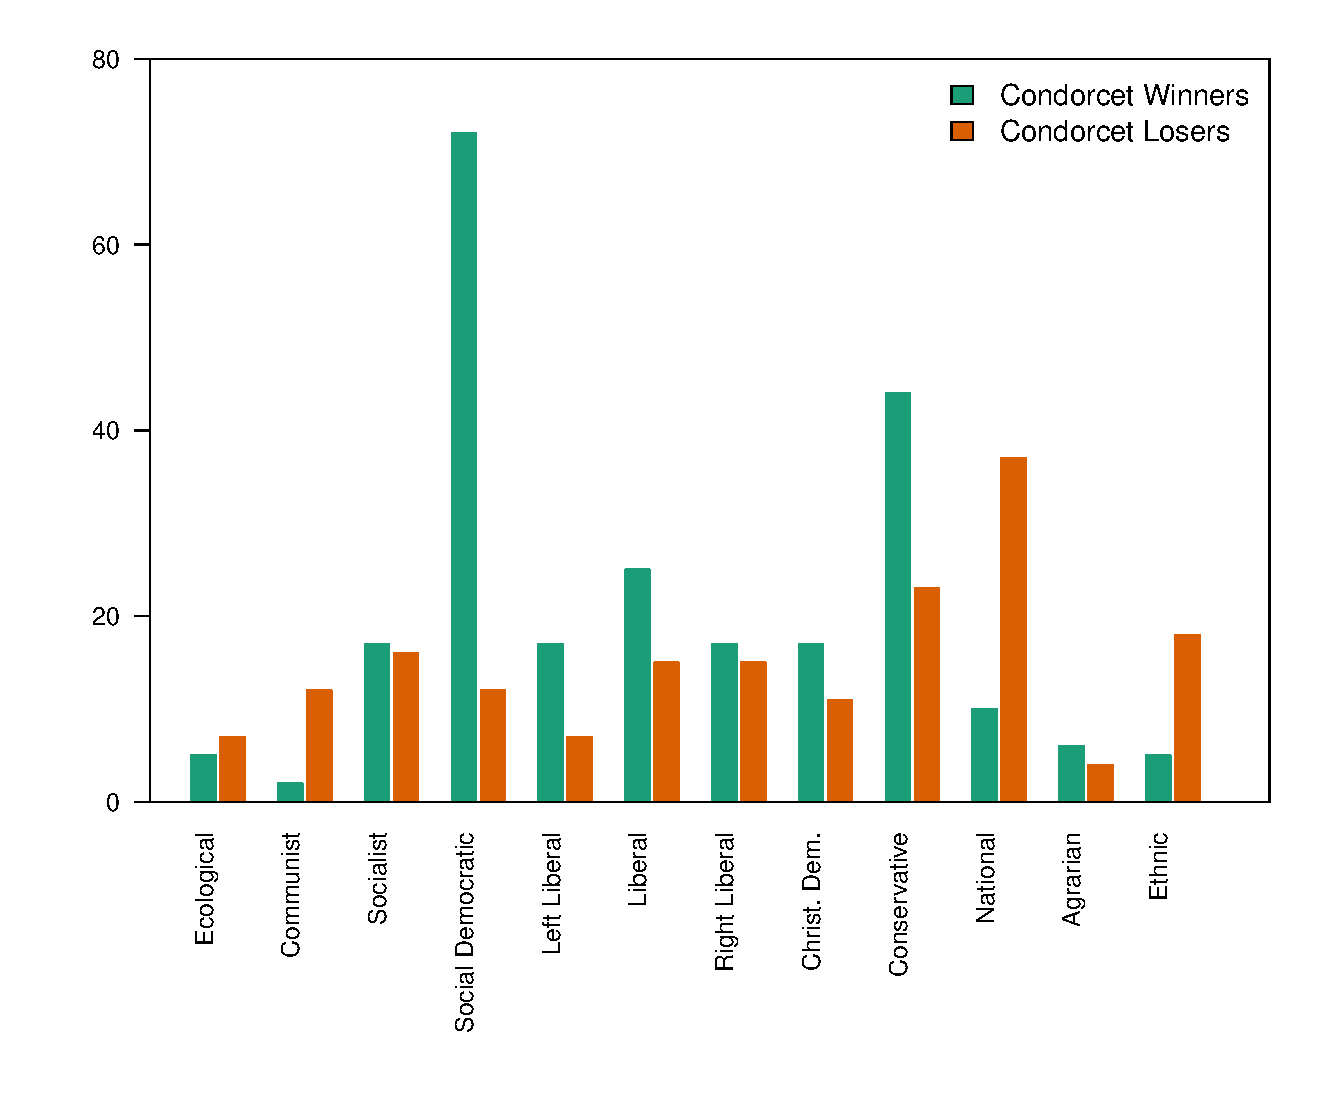
\includegraphics[width=.85\linewidth]{barplot.pdf}
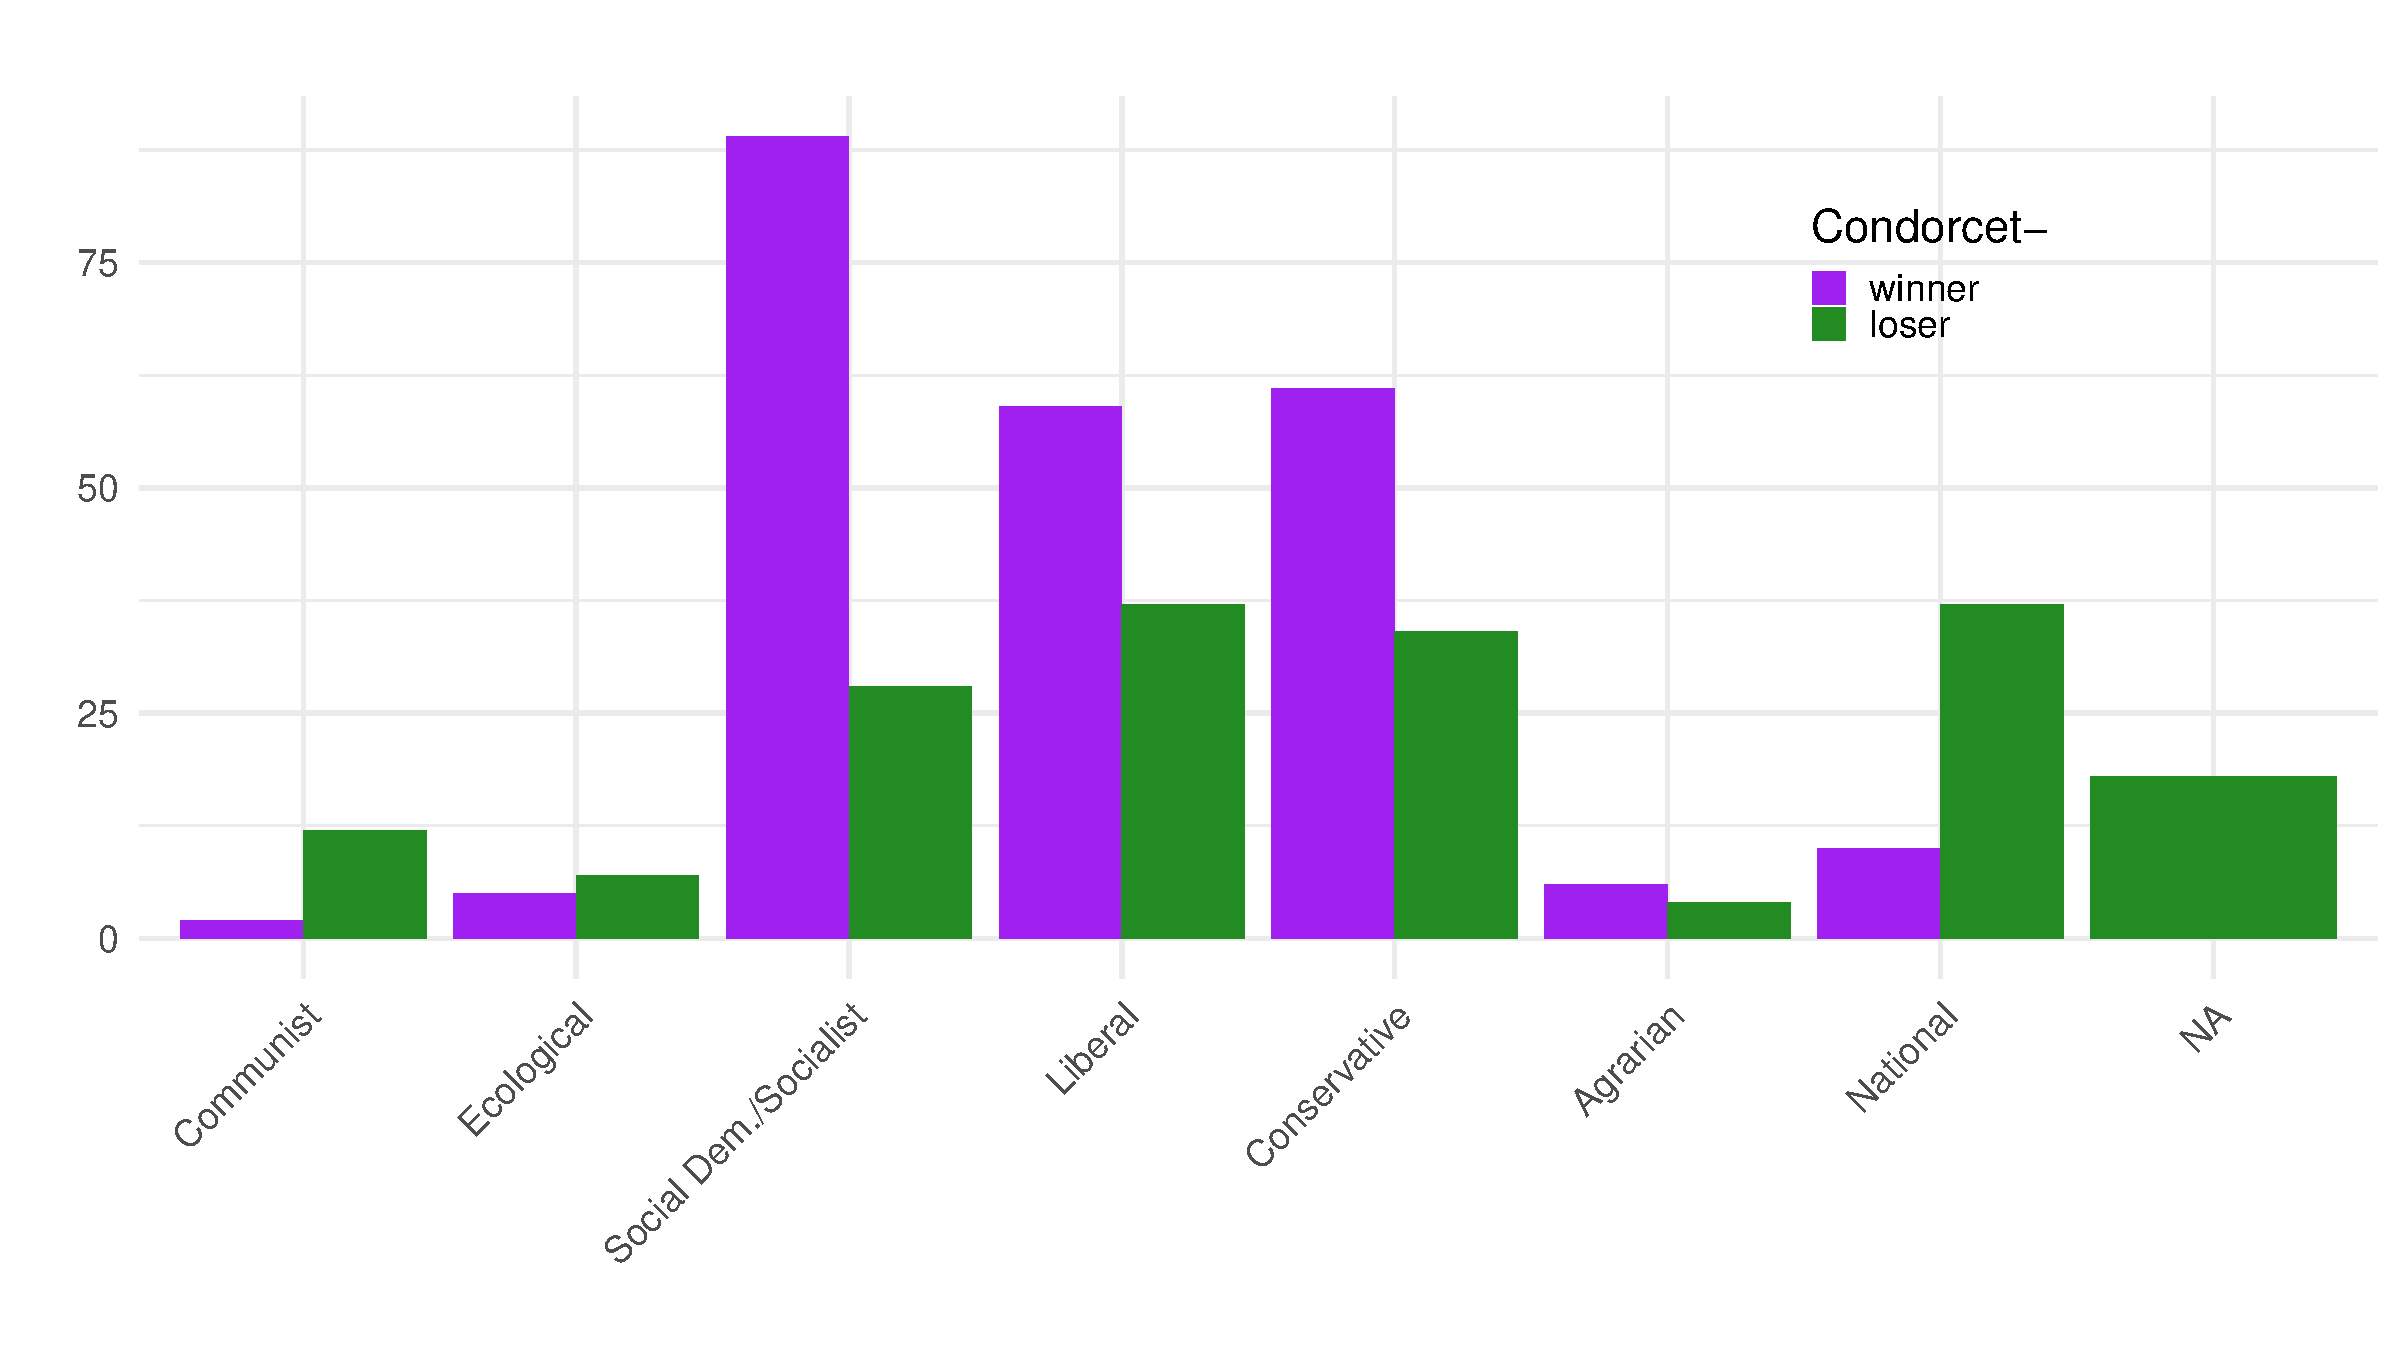
\includegraphics[width=\linewidth]{barplotFAM}
%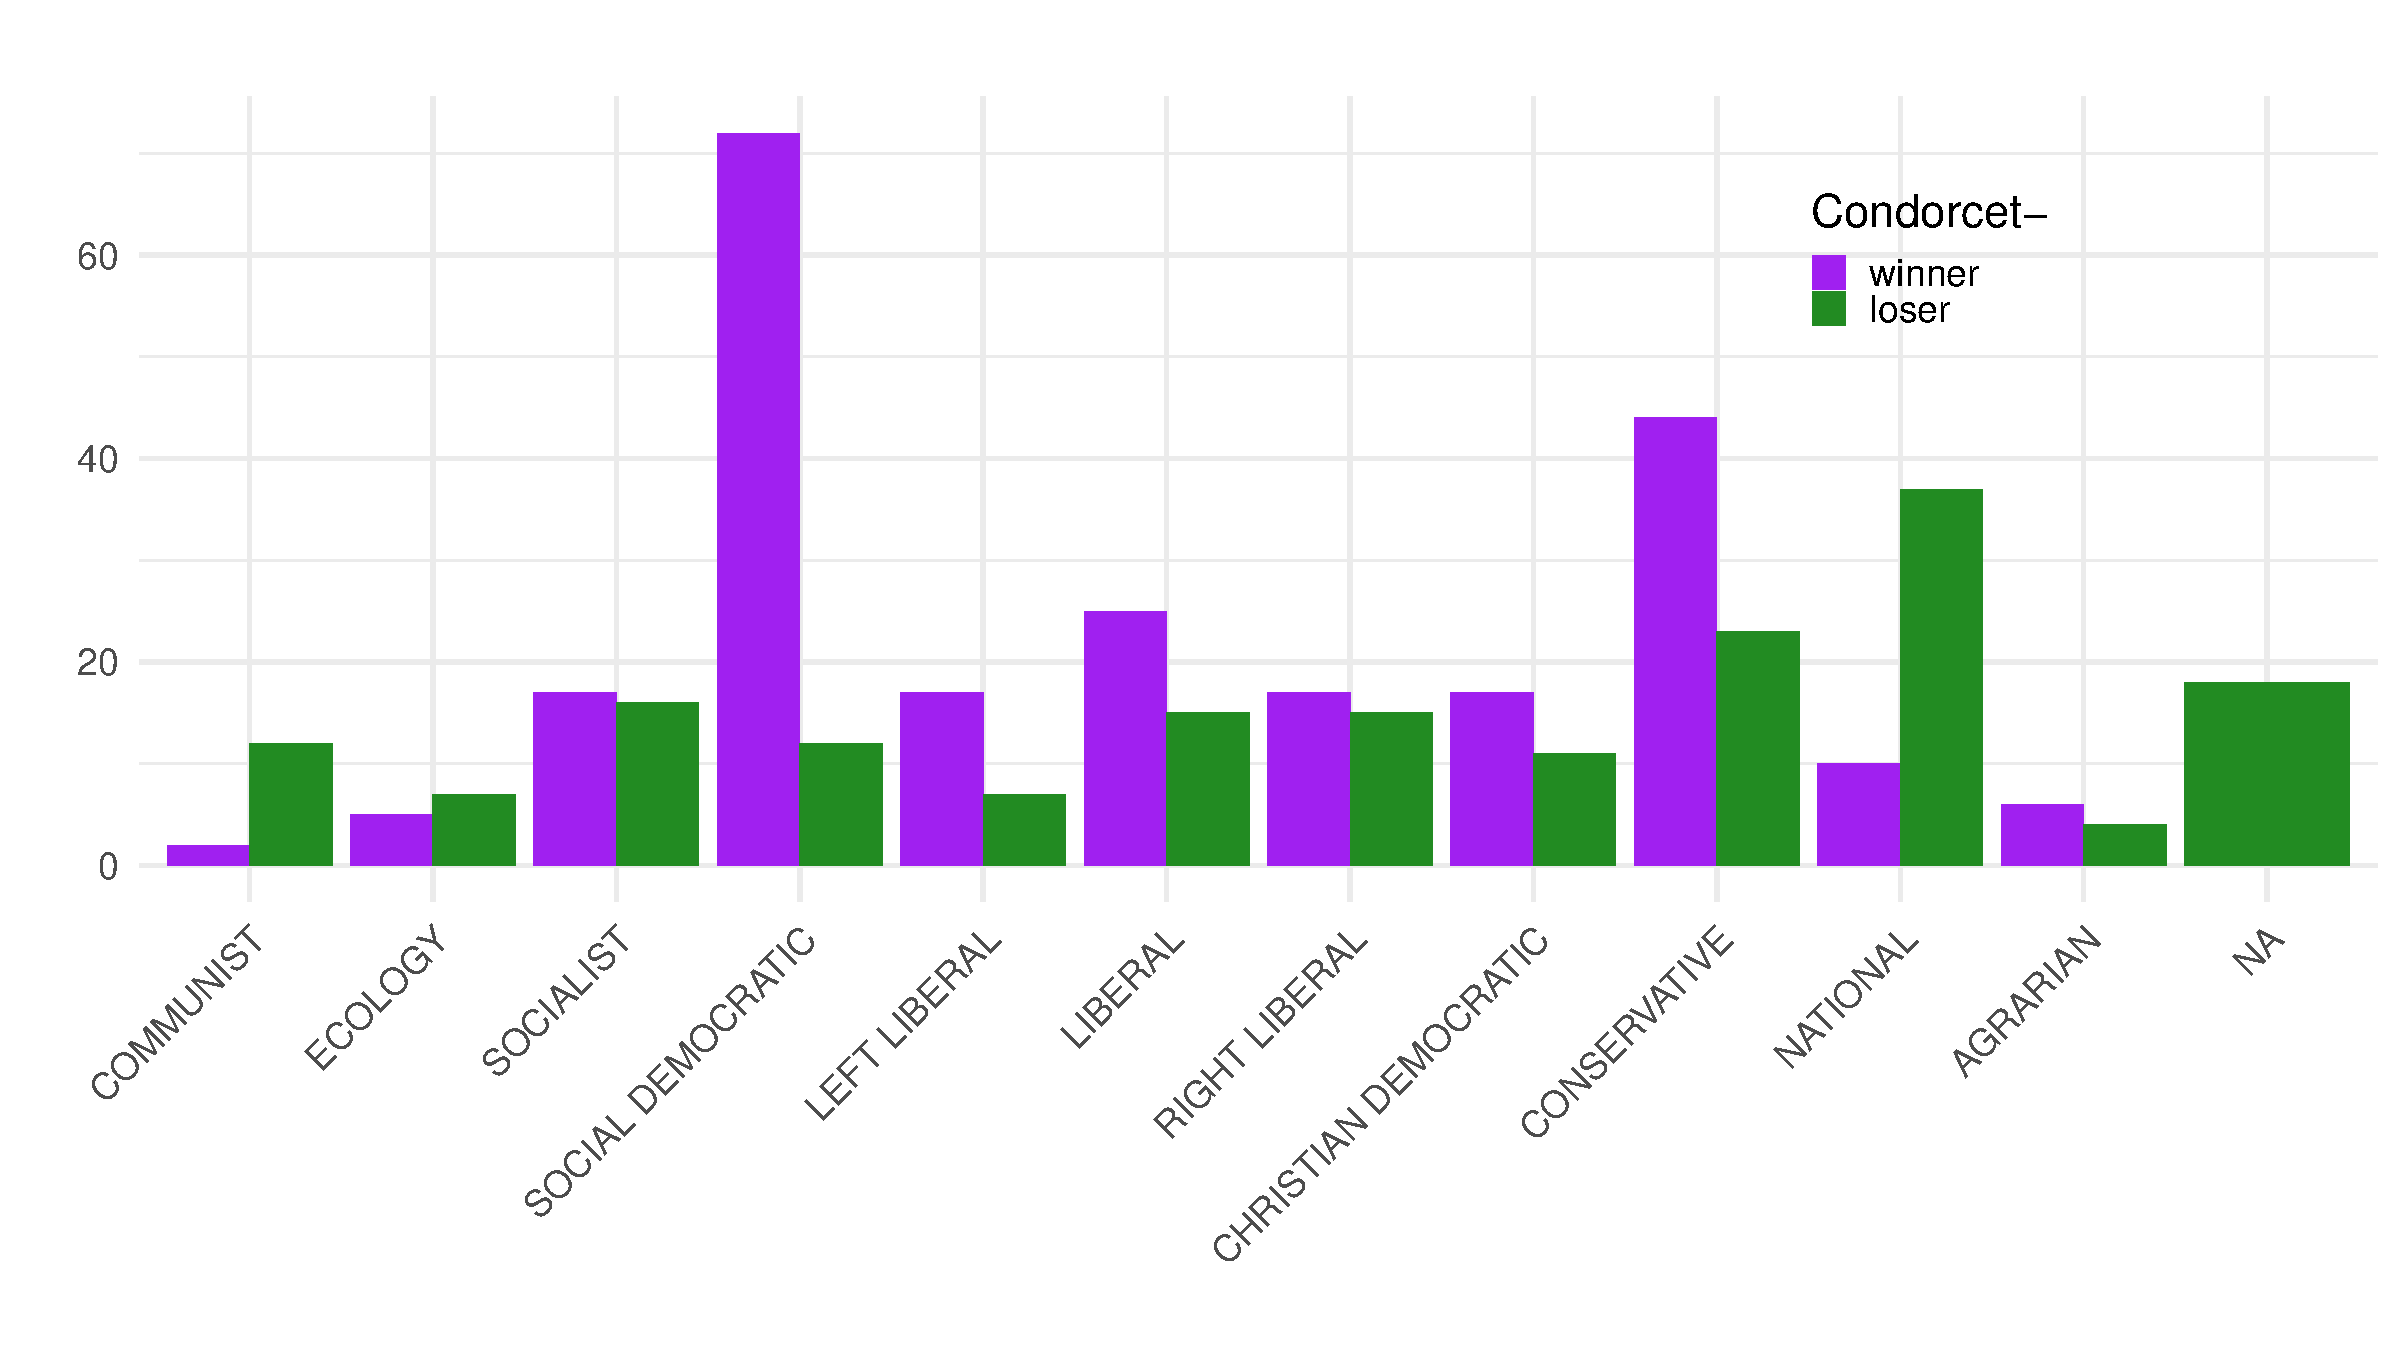
\includegraphics[width=\linewidth]{barplotraw}
\caption{Frequency of Condorcet winner and loser parties by party family \label{f1}}
\end{figure}

Given that Condorcet winners exist in virtually all of the elections under study, we subsequently focus on descriptive results on these winner parties and candidates. Figure \ref{f1} plots the frequency of Condorcet winners and losers by party family.\footnote{
  We use the classification of party families as provided by the CSES. It is based on expert judgments of the CSES national collaborators as to which ideological family each party belongs to. 
} It shows that Condorcet winners are most often social-democratic parties. National parties are the most common among the Condorcet losers. A full list of Condorcet winner and loser parties is presented in the (Online-)Appendix. Table \ref{tab.g7} provides an extract from the full list, covering the G7 countries only.

\begin{table}
\caption{List of Condorcet winner and loser parties/candidates in G7 countries}
\footnotesize{
\begin{tabular}{llll} \toprule 
Country & Year & Condorcet Winner Party & Condorcet Loser Party \\ \midrule 
  Canada & 1997 &   Liberal Party (LIB) &   Bloc Quebecois (BQ)   \\ 
  Canada & 2004 &   Liberal Party (LIB) &   Bloc Quebecois (BQ)   \\ 
  Canada & 2008 &   Conservative Party (CP) &   Bloc Quebecois (BQ)   \\ 
  Canada & 2011 &   Conservative Party (CP) &   Bloc Quebecois (BQ)   \\ 
  Canada & 2015 &   Liberal Party (LIB) &   Bloc Quebecois (BQ)   \\ 
  Canada & 2019 &   Liberal Party (LIB) &   Bloc Quebecois (BQ)   \\  \midrule
 France & 2002 & Jacques Chirac (PS) & Jean-Marie LePen (FN)\\ 
 France & 2012 &   Francois Hollande (PS)   &   Francois Bayrou (MoDem)  \\ 
 France & 2017 &   Emmanuel Macron (LaREM)    &   Marine Le Pen (FN) \\ \midrule 
 Germany & 1998 &        Soc. Dem. Party (SPD) &   Left Party (DIE LINKE)   \\ 
  Germany & 2002 &        Soc. Dem. Party (SPD) &   The Republicans (REP) \\ 
  Germany & 2005 &        Soc. Dem. Party (SPD) &   Nat. Dem. Party of Germ. (NPD) \\ 
  Germany & 2009 &   Christ. Dem. Party (CDU) &   Left Party (DIE LINKE)   \\ 
  Germany & 2013 &   Christ. Dem. Party (CDU) &   Alt. for Germany (AfD) \\ 
  Germany & 2017 &   Christ. Dem. Party (CDU) &   Alt. for Germany (AfD) \\ 
  Germany & 2021 &        Soc. Dem. Party (SPD) &   Alt. for Germany (AfD) \\  \midrule 
 Great Britain & 1997 &   Labor (Lab) &   Conservatives (Con) \\ 
  Great Britain & 2005 &   Labor (Lab) &   Conservatives (Con) \\ 
  Great Britain & 2015 &   Conservatives (Con) &   UK Independence Party (UKIP) \\ 
  Great Britain & 2017 &   Labor (Lab) &   Plaid Cymru (PC)   \\ 
  Great Britain & 2019 &   Conservatives (Con) &   Plaid Cymru (PC)   \\ \midrule
 Italy & 2006 &   National Alliance (AN)   &   Communist Refoundation (PRC) \\ 
  Italy & 2018 &   Five Star Movement (M5S) &   Free and Equal (LeU) \\ \midrule
  Japan & 1996 &   Liberal Democratic Party (LDP) &   New Party Harbinger (NPH) \\ 
  Japan & 2004 &   Democratic Party of Japan (DPJ)   &   Jap. Communist Party (JCP) \\ 
  Japan & 2007 &   Democratic Party of Japan (DPJ)   &   Jap. Communist Party (JCP) \\ 
  Japan & 2013 &   Lib. Dem. Party (LDP) &   Green Wind \\ 
  Japan & 2017 &   Lib. Dem. Party (LDP) &   Japanese Communist Party (JCP) \\ \midrule
  USA & 1996 & Democratic Party & Reform Party \\
  USA & 2004 & Democratic Party & Reform Party \\ 
% USA     & 1996 &   Bill Clinton (DEM)  & Bob Dole (GOP) \\ 
% USA     & 2008 &   Barack Obama (DEM)   &  John McCain (GOP)   \\ 
% USA     & 2012 &   Barack Obama (DEM)    &  Mitt Romney (GOP)    \\ 
% USA     & 2016 &  Hillary  Clinton (DEM)  &  Donald J. Trump (GOP)     \\ 
% USA    & 2020 & Joseph R. Biden Jr. (DEM)   &  Donald J. Trump (GOP)  \\   
\bottomrule
\end{tabular}	}
\label{tab.g7}
\end{table}

This list yields some interesting insights. For example, although Condorcet-winner parties are often centrally located within the party system, they are not necessarily large parties. In the Netherlands, for instance, the liberal party 'Democrats 66' (D66) was the Condorcet-winner party in 2010, 2017, and 2021, despite its low vote share of only 7\%, 12\%, and 15\%, respectively. In the 2010 election, it was only the sixth-largest party in terms of votes and parliamentary seats. In 2017, it ranked fourth, and in 2021, it ranked second. In an earlier study for the election year 1994 -- which our dataset does not extend back to -- \cite{vanDeemen1998} had already found that D66 emerged as the Condorcet-winner party. Even then, the vote share of 15.5\% did not reflect the broad support for the D66 party among the electorate. We also find a correspondence with the results from two Danish elections in 1998 and 2001, as identified by \cite{KurrildKlitgaard2008} (using a different dataset than the one we employed). 

For Great Britain, our data show that the Condorcet winners can indeed vary but generally align with the winners under the First-Past-The-Post system. An exception is 2017, when the Tories narrowly won the general election, but Labour emerged as the Condorcet winner. The 2005 election is not included in our dataset; however, \cite{Abramson2013} identified the Liberal-Democrats as the Condorcet winner for that election. Our (Online-)Appendix presents the values for all other countries.

Noteworthy, there are instances where Condorcet-loser parties gain a significant number of votes and seats. Polarising right-wing parties, in particular, benefit from this imbalance. For example, the far-right 'Sweden Democrats' were the Condorcet-loser party in 2006, 2014, and 2018. Yet, they increased their vote share to 12.9\% in the 2018 election, becoming the third-largest party out of eight in the 2014 and 2018 parliaments. In Germany, the far-right Condorcet loser AfD became the third-largest faction in the Bundestag in 2017 with 12.5\% of the vote, surpassing three parties that had each won their pairwise comparison against the AfD. An even more extreme case is the 2011 Swiss election, where the national-conservative Swiss People's Party gained the largest vote share while emerging as the Condorcet loser. 

Table \ref{tb.efficiency} provides a systematic overview of the empirical \textit{Condorcet efficiency}\footnote{
    The term Condorcet efficiency refers to the conditional probability that a voting rule selects the Condorcet winner, given that one exists \citep{Gehrlein1998}.
} of electoral systems. We calculate how frequently Condorcet winners emerge as electoral victors (i.e., as the largest parliamentary faction) and examine how often they are included in the subsequent government following the election. The results are presented by election type and electoral system. At the end of this section, we also report the Condorcet efficiencies of the Borda count. The first row of Table \ref{tb.efficiency} highlights the frequency\footnote{
    The values in square brackets indicate the confidence interval of Agresti-Coull binomial tests \citep{Agresti1998} (values in percentages and at a 90\% significance level).
} at which Condorcet winners become the largest electoral party, revealing significant variation across election types and systems. Condorcet winners are most successful in  parliamentary elections with mixed electoral systems (82\%) and in presidential elections (79\%), but their success rate is lowest in parliamentary elections using proportional representation (61\%). 

\begin{table}[ht]
\caption{Condorcet efficiency by type of election (parliamentary vs. presidential and by electoral systems.}
\centering
\begin{tabular}{l|rrr|r} \toprule 
 %  & \multicolumn{4}{c}{Type of election and electoral system}\\
   & \multicolumn{3}{c|}{\textbf{Parliamentary}} & \textbf{Presidential}\\
 Condorcet Winner& Plurality  & Proportional & Mixed &  \\
                &   $N=26$   & $N=135$   & $N=51$    & $N=41$ \\ \midrule 
largest elect.& 71\%     & 62\%   &   81\% &  79\%  \\
party / candidate & \emph{[56-83]} & \emph{[54-68]} & \emph{[70-88]} & \emph{[71-89]} \\ \midrule 
% party/candidate  &  (20/28) &  (82/133) &  (39/48) &  (37/45) \\ \midrule 
   prime minister/ &   92\% &  66\% &   73\% &   78\% \\
president & \emph{[71-92]} & \emph{[48-63]} & \emph{[61-82]} & \emph{[71-90]} \\ \midrule
%  president         &  (25/28) & (76/115) &  (35/48) &  (37/45) \\  \midrule
part of &   96\% &  88\% &   98\% &    \\
government & \emph{[86-100]} & \emph{[82-92]} & \emph{[91-100]} & \\ \midrule
%  government &  (29/30) & (119/135) &  (50/51) &   \\ \midrule
Condorcet Loser & & & & \\
part of & 0\%& 13\%& 6\% & 2\%\\
government / president &  & \emph{[11-22]} & \emph{[2-19]} & \emph{[0-12]} \\
%government/president & (0/20) & (18/112) & (3/37) & (2/47) \\
\bottomrule 
\end{tabular}
\label{tb.efficiency}
\end{table}
 
The second row in Table \ref{tb.efficiency} reports how often Condorcet winners win the prime minister's office or the presidency. It shows that in parliamentary systems with plurality or proportional rules, Condorcet winners obtain government leadership even if they are not the largest electoral party, increasing their success rate to 88\% resp. 66\%. This is not the case in any of the mixed systems in our data.  Since the most-vote getter in presidential elections typically also win the presidency, the rate is identical to the first row. Our findings concerning parliamentary elections align with those of \cite{Desai2025}, who used OLS regressions to show that weak Condorcet winners (core parties) are about 24 percentage points more likely to appoint the prime minister, with even higher probabilities for strong Condorcet winners.

Condorcet winners may still hold government offices, e.g., as a junior coalition partner. The results reported in the third row indicate that this is often the case: the government participation rates are significantly larger than the election winner rates and the prime minister/presidency rates. Again, there is variation by election type and system, with  mixed electoral systems in parliamentary elections showing the largest Condorcet efficiency in government participation (98\%). Proportional and mixed rules in parliamentary elections are less efficient in selecting Condorcet winners into government  (92\% and 89\%). Overall, the government formation period that follows upon parliamentary elections enhances the Condorcet efficiency of parliamentary systems, superseding presidential elections in terms of government posts for Condorcet winners.

Another way to assess the Condorcet efficiency of electoral systems is to examine how frequently the participation of Condorcet-loser parties in government is prevented. The bottom row in Table \ref{tb.efficiency} indicates that proportional electoral systems are most prone to the success (viz., becoming part of the government) of Condoret loser parties. From a normative standpoint, this may be justified, as one of the premises of proportional systems is to enable ethnic, religious or other minorities to have their legitimate share of power, so as to prevent the 'tyranny of the majority'. However, in only four out of twenty cases the Condorcet loser party in cabinet is categorized as ethnic party. 

A particularly striking scenario in candidate elections, which defies axiomatically grounded reasoning, occurs when, ironically, the Condorcet loser emerges as the plurality winner. This phenomenon is know as \textit{Borda paradox}, termed after Condorcet's intellectual foil. In our analysis of \nbelections presidential candidate elections, we uncover a notable instance of this paradox in the 2000 Mexican presidential election. In this case, Vicente Fox secured the plurality vote despite being a Condorcet loser, while the Condorcet winner, Cuauhtémoc Cárdenas Solórzano, placed third in the election.

Finally, we applied our data to the Borda rule, a positional voting system that assigns weights to alternatives based on their rank-order positions. We then compared the winners under the Borda rule with the Condorcet winner to evaluate how often they align. The results reveal that 93.4\% of Borda winners are also Condorcet winners, indicating that the Borda rule achieves a higher Condorcet efficiency compared to the plurality rule (see Table \ref{tb.efficiency}).

If a party is the Borda winner but not the Condorcet winner, this discrepancy stems from differences in the intensity of preferences. The Condorcet method adheres to Arrow's Independence of Irrelevant Alternatives (IIA), which disregards any consideration of preference intensities \citep[Ch.~7]{Sen2017}. In contrast, the Borda rule incorporates preference intensities through ordinal information \citep{Maskin2024}. For example, suppose 60\% of the electorate prefers $A \succ B \succ C$, while 40\% prefers $B \succ C \succ A$. In this scenario, $A$ emerges as the Condorcet winner, while $B$ becomes the Borda winner. This outcome is influenced by candidate $C$ (violating IIA): their middle ranking within the minority group may indicate that the preference intensity for $B$ over $A$ in the smaller group outweighs the preference intensity for $A$ over $B$ in the majority group.

When the Condorcet winner belongs to the socialist/social democratic or liberal party families, they also tend to be the Borda winner in 98\% of cases. In contrast, this coincidence is lower for the conservative/Christian democratic party family, at 85\%. 

\section{Conclusion}
Two hundred and forty years ago, the Marquis de Condorcet introduced the paradox that now bears his name to the French Academy of Sciences. Ever since, it has been recognized as a profound challenge within the social sciences. In recent decades, researchers have sought in various ways to assess the empirical relevance of the Condorcet paradox. However, it has always been clear that only a comprehensive empirical analysis across different countries and dates could provide a substantive insight. This study leverages the availability of comparative data and advanced computational capabilities to conduct the first empirical investigation in this broader vein. Our findings reveal that the Condorcet paradox holds virtually no empirical relevance.

We find a Condorcet winner in almost every country and at almost every point in time. Moreover, we are able to identify who these Condorcet winners are and the party families to which they belong. Our results are encouraging in that Condorcet winners frequently succeed in becoming part of the governing coalitions. However, the degree of Condorcet efficiency varies significantly between electoral systems.

Our analysis also demonstrates that Condorcet losers nearly always exist. Fortunately, Condorcet-loser parties do not frequently make it into government. However, we observe that different electoral systems vary in their effectiveness at preventing this. Our findings reveal that proportional electoral rules are the least effective in ensuring electoral victory and government participation for Condorcet winners, while simultaneously being the least effective at preventing Condorcet losers from participating in government. These insights should be carefully considered in ongoing debates about electoral reform.

Moreover, our work can be understood as academic endorsement for advocates of electoral reforms favouring the Condorcet method \citep{Maskin2016, Maskin2017, Maskin2017a}. While these advocates emphasise its axiomatic advantages, they are, of course, mindful of the paradox's challenges. Our findings suggest that, in weighing the strengths and weaknesses of the Condorcet method, its principal shortcoming should not be overemphasized. In this sense, this study aims not only to make an academic contribution but also to inform and inspire current and future debates on electoral reform.

%\newpage 
\singlespacing
%\bibliographystyle{abbrvnat}
\bibliographystyle{ejbib}
\bibliography{CondorcetCycle}
%\input{EJSubm.bbl}

%%%%%%%%%%%%%%%%%%%%%%%%%%%%%%%%%%%%%%%%%%
\appendix
\section*{Appendices}

Note: The appendix is  proposed to be published online. We add the appendices to the main text in line with the submission guidelines. 

\singlespacing
\newpage
%%%%%%%%%%%%%%%%%%%%%%%%%%%
\begin{landscape}
\section{Countries and Election Years Included in Analysis}
\tiny{
\begin{longtable}{|r|r|r|r|r|r|r|r|r|r|r|r|r|r|r|r|r|r|r|r|r|r|r|r|r|r|r|} \toprule 
			%		\begin{scriptsize}
				%\centering
    & '96 & '97 & '98 & '99 & '00 & '01 & '02 & '03 & '04 & '05 & '06 & '07 & '08 & '09 & '10 & '11 & '12 & '13 & '14 & '15 & '16 & '17 & '18 & '19 & '20 & '21\\ \midrule \endfirsthead \midrule
    & '96 & '97 & '98 & '99 & '00 & '01 & '02 & '03 & '04 & '05 & '06 & '07 & '08 & '09 & '10 & '11 & '12 & '13 & '14 & '15 & '16 & '17 & '18 & '19 & '20 & '21\\ \midrule \endhead \midrule \endfoot
\bottomrule	\endlastfoot
Albania &     &     &     &     &     &     &     &     &     &    x &     &     &     &     &     &     &     &     &     &     &     &    x &     &     &     &     \\  \midrule
Argentina &     &     &     &     &     &     &     &     &     &     &     &     &     &     &     &     &     &     &     &    x &     &     &     &     &     &     \\ \midrule
Australia &    x &     &     &     &     &     &     &     &    x &     &     &    x &     &     &     &     &     &    x &     &     &     &     &     &    x &     &     \\ \midrule
Austria &     &     &     &     &     &     &     &     &     &     &     &     &    x &     &     &     &     &    x &     &     &     &    x &     &     &     &     \\ \midrule
Belarus &     &     &     &     &     &    x &     &     &     &     &     &     &    x &     &     &     &     &     &     &     &     &     &     &     &     &     \\ \midrule
Belgium &     &     &     &    x &     &     &     &    x &     &     &     &     &     &     &     &     &     &     &     &     &     &     &     &    x &     &     \\ \midrule
Brazil &     &     &     &     &     &     &    x &     &     &     &    x &     &     &     &    x &     &     &     &    x &     &     &     &    x &     &     &     \\ \midrule
Bulgaria &     &     &     &     &     &    x &     &     &     &     &     &     &     &     &     &     &     &     &    x &     &     &     &     &     &     &     \\ \midrule
Canada &     &    x &     &     &     &     &     &     &    x &     &     &     &    x &     &     &    x &     &     &     &    x &     &     &     &    x &     &     \\ \midrule
Chile &     &     &     &    x &     &     &     &     &     &    x &     &     &     &    x &     &     &     &     &     &     &     &    x &     &     &     &     \\ \midrule
Costa Rica &     &     &     &     &     &     &     &     &     &     &     &     &     &     &     &     &     &     &     &     &     &     &    x &     &     &     \\ \midrule
Croatia &     &     &     &     &     &     &     &     &     &     &     &    x &     &     &     &     &     &     &     &     &     &     &     &     &     &     \\ \midrule
Czech Republic &    x &     &     &     &     &     &    x &     &     &     &    x &     &     &     &    x &     &     &    x &     &     &     &     &     &     &     &     \\ \midrule
Czechia &     &     &     &     &     &     &     &     &     &     &     &     &     &     &     &     &     &     &     &     &     &    x &     &     &     &    x \\ \midrule
Denmark &     &     &    x &     &     &    x &     &     &     &     &     &    x &     &     &     &     &     &     &     &     &     &     &     &    x &     &     \\ \midrule
El Salvador &     &     &     &     &     &     &     &     &     &     &     &     &     &     &     &     &     &     &     &     &     &     &     &    x &     &     \\ \midrule
Estonia &     &     &     &     &     &     &     &     &     &     &     &     &     &     &     &    x &     &     &     &     &     &     &     &     &     &     \\ \midrule
Finland &     &     &     &     &     &     &     &    x &     &     &     &    x &     &     &     &    x &     &     &     &    x &     &     &     &    x &     &     \\ \midrule
France &     &     &     &     &     &     &    x &     &     &     &     &    x &     &     &     &     &    x &     &     &     &     &    x &     &     &     &     \\ \midrule
Germany &     &     &    x &     &     &     &    x &     &     &    x &     &     &     &    x &     &     &     &    x &     &     &     &    x &     &     &     &    x \\ \midrule
Great Britain &     &    x &     &     &     &     &     &     &     &    x &     &     &     &     &     &     &     &     &     &    x &     &    x &     &    x &     &     \\ \midrule
Greece &     &     &     &     &     &     &     &     &     &     &     &     &     &    x &     &     &    x &     &     &   2 &     &     &     &    x &     &     \\ \midrule
Hong Kong &     &     &    x &     &    x &     &     &     &    x &     &     &     &    x &     &     &     &    x &     &     &     &    x &     &     &     &     &     \\ \midrule
Hungary &     &     &    x &     &     &     &    x &     &     &     &     &     &     &     &     &     &     &     &     &     &     &     &    x &     &     &     \\ \midrule
Iceland &     &     &     &    x &     &     &     &    x &     &     &     &    x &     &    x &     &     &     &    x &     &     &    x &    x &     &     &     &     \\ \midrule
India &     &     &     &     &     &     &     &     &     &     &     &     &     &     &     &     &     &     &     &     &     &     &     &    x &     &     \\ \midrule
Ireland &     &     &     &     &     &     &    x &     &     &     &     &    x &     &     &     &    x &     &     &     &     &    x &     &     &     &     &     \\ \midrule
Israel &    x &     &     &     &     &     &     &    x &     &     &    x &     &     &     &     &     &     &    x &     &     &     &     &     &     &    x &     \\ \midrule
Italy &     &     &     &     &     &     &     &     &     &     &    x &     &     &     &     &     &     &     &     &     &     &     &    x &     &     &     \\ \midrule
Japan &    x &     &     &     &     &     &     &     &    x &     &     &    x &     &     &     &     &     &    x &     &     &     &    x &     &     &     &     \\ \midrule
Kenya &     &     &     &     &     &     &     &     &     &     &     &     &     &     &     &     &     &    x &     &     &     &     &     &     &     &     \\ \midrule
Latvia &     &     &     &     &     &     &     &     &     &     &     &     &     &     &    x &    x &     &     &    x &     &     &     &    x &     &     &     \\ \midrule
Lithuania &     &    x &     &     &     &     &     &     &     &     &     &     &     &     &     &     &     &     &     &     &    x &     &     &     &    x &     \\ \midrule
Mexico &     &    x &     &     &    x &     &     &    x &     &     &    x &     &     &    x &     &     &    x &     &     &    x &     &     &    x &     &     &     \\ \midrule
Montenegro &     &     &     &     &     &     &     &     &     &     &     &     &     &     &     &     &    x &     &     &     &    x &     &     &     &     &     \\ \midrule
Netherlands &     &     &    x &     &     &     &    x &     &     &     &    x &     &     &     &    x &     &     &     &     &     &     &    x &     &     &     &    x \\ \midrule
New Zealand &    x &     &     &     &     &     &    x &     &     &     &     &     &    x &     &     &    x &     &     &    x &     &     &    x &     &     &    x &     \\ \midrule
Norway &     &    x &     &     &     &    x &     &     &     &    x &     &     &     &    x &     &     &     &    x &     &     &     &    x &     &     &     &     \\ \midrule
Peru &     &     &     &     &    x &    x &     &     &     &     &    x &     &     &     &     &    x &     &     &     &     &    x &     &     &     &     &    x \\ \midrule
Philippines &     &     &     &     &     &     &     &     &    x &     &     &     &     &     &    x &     &     &     &     &     &    x &     &     &     &     &     \\ \midrule
Poland &     &    x &     &     &     &    x &     &     &     &    x &     &    x &     &     &     &    x &     &     &     &     &     &     &     &    x &     &     \\ \midrule
Portugal &     &     &     &     &     &     &    x &     &     &    x &     &     &     &    x &     &     &     &     &     &    x &     &     &     &    x &     &     \\ \midrule
Rep. of Korea &     &     &     &     &    x &     &     &     &    x &     &     &     &    x &     &     &     &    x &     &     &     &    x &     &     &     &     &     \\ \midrule
Romania &    x &     &     &     &     &     &     &     &    x &     &     &     &     &    x &     &     &    x &     &    x &     &    x &     &     &     &     &     \\\midrule
Russian Fed. &     &     &     &      &    x &     &     &     &      &     &     &     &     &     &     &     &     &     &     &     &     &     &     &     &     &     \\ \midrule
Serbia &     &     &     &     &     &     &     &     &     &     &     &     &     &     &     &     &    x &     &     &     &     &     &     &     &     &     \\ \midrule
Slovakia &     &     &     &     &     &     &     &     &     &     &     &     &     &     &    x &     &     &     &     &     &    x &     &     &     &    x &     \\ \midrule
Slovenia &    x &     &     &     &     &     &     &     &    x &     &     &     &    x &     &     &    x &     &     &     &     &     &     &     &     &     &     \\ \midrule
South Africa &     &     &     &     &     &     &     &     &     &     &     &     &     &    x &     &     &     &     &    x &     &     &     &     &     &     &     \\ \midrule
Spain &    x &     &     &     &    x &     &     &     &    x &     &     &     &    x &     &     &     &     &     &     &     &     &     &     &     &     &     \\ \midrule
Sweden &     &     &    x &     &     &     &    x &     &     &     &    x &     &     &     &     &     &     &     &    x &     &     &     &    x &     &     &     \\ \midrule
Switzerland &     &     &     &    x &     &     &     &    x &     &     &     &    x &     &     &     &    x &     &     &     &     &     &     &     &     &     &     \\ \midrule
Taiwan &    x &     &     &     &     &    x &     &     &    x &     &     &     &    x &     &     &     &    x &     &     &     &    x &     &     &     &    x &     \\ \midrule
Thailand &     &     &     &     &     &    x &     &     &     &     &     &    x &     &     &     &    x &     &     &     &     &     &     &     &    x &     &     \\ \midrule
Tunisia &     &     &     &     &     &     &     &     &     &     &     &     &     &     &     &     &     &     &     &     &     &     &     &    x &     &     \\ \midrule
Turkey &     &     &     &     &     &     &     &     &     &     &     &     &     &     &     &    x &     &     &     &    x &     &     &    x &     &     &     \\ \midrule
Ukraine &     &     &    x &     &     &     &     &     &     &     &     &     &     &     &     &     &     &     &     &     &     &     &     &     &     &     \\ \midrule
USA &    x &     &     &     &     &     &     &     &    x &     &     &     &    x &     &     &     &    x &     &     &     &    x &     &     &     &    x &     \\ \midrule
Uruguay &     &     &     &     &     &     &     &     &     &     &     &     &     &    x &     &     &     &     &     &     &     &     &     &    x &     &     \\   \bottomrule
%\end{tabular}
		\end{longtable} }

        %\end{scriptsize}
\end{landscape}
	
%%%%%%%%%%%%%%%%%%%%%%%%%%%%%%%%%%%	
\section{Full List of Condorcet Winner and Condorcet Loser Parties in Parliamentary Elections}
%	
\scriptsize{
\begin{longtable}{|l|c|l|l|}  \toprule 
	\textbf{Country} & \textbf{Year} & \textbf{Condorcet winner candidate/party} & \textbf{Condorcet loser candidate/party} \\ \midrule 	\endfirsthead	\midrule
\textbf{Country} & \textbf{Year} & \textbf{Condorcet winner party} & \textbf{Condorcet loser party} \\		\midrule \endhead \midrule \endfoot \bottomrule
\endlastfoot \midrule
Albania & 2005 &   Democratic Party of Albania (PD) &   Agrarian Party (PAA) \\ 
Albania & 2017 &   Socialist Party of Albania (PS) &   Libra Party (LIBRA) \\ 
%
Argentina & 2015 &   Front for the Victory (FPV) &   Progressives (Pro) \\ 
%
Australia & 1996 &   Liberal Party (LP) &    Australian Greens (AG) \\ 
Australia & 2004 &   Liberal Party (LP) &   One Nation Party (ONP) \\ 
Australia & 2007 &   Australian Labor Party (ALP)  &   National Party of Australia (NPA)      \\ 
Australia & 2013 &   Liberal Party (LP) &   Australian Greens (AG) \\ 
Australia & 2019 &   Liberal Party (LP) &   One Nation Party (ONP) \\ 
%
Austria & 2008 &   Soc. Dem. Party of Austria (SPÖ) &   Dinkhauser List  \\ 
Austria & 2013 &   Soc. Dem. Party of Austria (SPÖ) &   Alliance for the Future of   \\ 
    &  &   &     Austria (BZÖ) \\ 
Austria & 2017 &   Austrian People's Party (OVP)   &   Peter Pilz List (PILZ) \\ 
%
Belarus & 2001 &   Communist Party of Belarus  &   United Civil Party  \\ 
Belarus & 2008 &   The BNF Party  &   United Civil Party  \\  
%
Belgium-Flanders & 1999 & Live Differently (AGALEV)  /  &  Flemish Block/ \\ 
   &   &   Green  &   Importance (VB)\\ 
Belgium-Wallonia & 1999 & Confederated Ecologists (ECOLO)   &  National Front (FN)   \\ 
  Belgium & 2003 &   Socialist Party Differently (SP)   &   Confederated Ecologists (ECOLO)   \\ 
Belgium-Flanders & 2019 & Christian Democratic -   &  Flemish Block  (VB)\\ 
 &  & Flemish (CD-V) &   \\ 
Belgium-Wallonia & 2019 &  Confederated Ecologists (ECOLO) &  People's Party (PP)\\ 
%
Brazil & 2002 &   Workers Party (PT) &   Brazilian Labor Party (PTB) \\ 
  Brazil & 2006 &   Workers Party (PT) &   Brazilian Labor Party (PTB) \\ 
Brazil & 2010 &   Workers Party (PT) &   Democrats (DEM)  \\ 
Brazil & 2014 &   Workers Party (PT) &   Republic Party (PR)   \\ 
Brazil & 2018 &   Workers Party (PT) &   Brazilian Republican Party (PRB)  \\ 
%
Bulgaria & 2001 &   National Movement for   &   Euroleft (BE) \\ 
    &   &    Stability and Progress (NDS) &    \\ 
Bulgaria & 2014 &   Citizens for European Development   &   Movement for Rights and   \\ 
    &   &    of Bulgaria (GERB) &     and Freedoms (DPS) \\ 
%
Canada & 1997 &   Liberal Party (LIB) &   Bloc Quebecois (BQ)   \\ 
Canada & 2004 &   Liberal Party (LIB) &   Bloc Quebecois (BQ)   \\ 
Canada & 2008 &   Conservative Party (CP) &   Bloc Quebecois (BQ)   \\ 
  Canada & 2011 &   Conservative Party (CP) &   Bloc Quebecois (BQ)   \\ 
Canada & 2015 &   Liberal Party (LIB) &   Bloc Quebecois (BQ)   \\ 
Canada & 2019 &   Liberal Party (LIB) &   Bloc Quebecois (BQ)   \\ 
%
Chile & 2005 &   Party for Democracy (PPD) &   Independent Democratic Union (UDI) \\ 
  Chile & 2009 &   Christian Democratic Party (PDC) &   Communist Party of Chile (PCCh) \\ 
Chile & 2017 &   National Renewal (RN) &   Political Evolution (Evopoli) \\ 
%
Costa Rica & 2018 &   Citizens' Action Party (PAC) &   Social Christian Republican \\ 
               &      &       &    Party (PRSC)  \\ 
%
Croatia & 2007 &   Croatian Democratic Union (HDZ) &   Croatian Democratic Alliance of   \\ 
          &      &    &   Slavonia and Baranja (HDSSB) \\ 
%
Czech Republic & 1996 &   Civic Democratic Party   &   Communist Party of Bohemia   \\ 
                 &   &     (ODS) &     and Moravia (KSCM) \\ 
Czech Republic  & 2002 &   Czech Social Democratic  &   Communist Party of Bohemia  \\ 
   &   &   Party (CSSD) & and Moravia (KSCM) \\ 
Czech Republic & 2006 &   Green Party (SZ) &   Communist Party of Bohemia   \\ 
                 &   &     &  and Moravia (KSCM) \\ 
Czech Republic  & 2010 &   Public Affairs (VV) &   Communist Party of Bohemia   \\ 
   &  &  & and Moravia (KSCM) \\ 
Czech Republic  & 2013 &   Action of Dissatisfied Citizens (ANO)   &   Civic Democratic Party (ODS)   \\
Czech Republic   & 2017 &   Action of Dissatisfied Citizens (ANO)  &   TOP 09 (TOP 09) \\ 
Czech Republic & 2021 &   Action of Dissatisfied Citizens (ANO)   &   Czech Pirate Party (Pirati)  \\ 
%
Denmark & 1998 &   Social Democrats (Sd) &   Danish People's Party (DF) \\ 
Denmark & 2001 &   Venstre, Denmark's Liberal &   Unity List - Red-Green  \\ 
  &  &    Party (V) &     Alliance (EL) \\ 
Denmark & 2007 &   Social Democrats (Sd) &   Unity List - Red-Green   \\ 
    &       &     &     Alliance (EL) \\ 
Denmark & 2019 &   Social Democrats (Sd) &   The New Right (NB) \\ 
%
Estonia & 2011 &        Social Democratic Party (SDE) &   Estonian People's Union (ER a)  \\ 
  Finland & 2003 &        Social Democratic Party of &   Swedish People's Party in   \\ 
           &   &          Finland (SDP) &   Finland (RKP - SFP) \\ 
  Finland & 2007 &   Center Party of Finland (KESK) &   Left Alliance (VAS) \\ 
  Finland & 2011 &        Social  Democratic Party of   &   Christian Democrats   \\ 
         &       &         Finland (SDP) &     (KD) \\ 
  Finland & 2015 &   Center Party of Finland (KESK) & --- \\ 
  Finland & 2019 &        Social Democratic Party of   &   Blue Reform (SIN)   \\ 
           &    &          Finland (SDP) &      \\ 
France & 2007 &   Union for a Popular Movement (UMP)     &   National Front (FN) \\ 
Germany & 1998 &        Social Democratic Party (SPD) &   Left Party (DIE LINKE)   \\ 
Germany & 2002 &        Social Democratic Party (SPD) &   The Republicans (REP) \\ 
Germany & 2005 &        Social Democratic Party (SPD) &   National Democratic Party (NPD)   \\ 
Germany & 2009 &   Christian Democratic Party (CDU) &   Left Party (DIE LINKE)   \\ 
Germany & 2013 &   Christian Democratic Party (CDU) &   Alternative for Germany (AfD) \\ 
Germany & 2017 &   Christian Democratic Party (CDU) &   Alternative for Germany (AfD) \\ 
Germany & 2021 &        Social Democratic Party (SPD) &   Alternative for Germany (AfD) \\ 
Great Britain & 1997 &   Labor (Lab) &   Conservatives (Con) \\ 
Great Britain & 2005 &   Labor (Lab) &   Conservatives (Con) \\ 
Great Britain & 2015 &   Conservatives (Con) &   United Kingdom Independence  \\ 
    &   &     &    Party (UKIP) \\ 
  Great Britain & 2017 &   Labor (Lab) &   Plaid Cymru (PC)   \\ 
  Great Britain & 2019 &   Conservatives (Con) &   Plaid Cymru (PC)   \\ 
  Greece & 2009 & Pan-Hellenic Socialist   &  Popular Orthodox Rally  \\ 
          &    & Movement (PASOK) &   (La.O.S)\\ 
  Greece & 2012 & Democratic Left (DIMAR) &  Golden Dawn (LS - XA) \\ 
  Greece & 2015 & Coalition of the Radical Left   &Golden Dawn (LS - XA)   \\ 
          &     &   (SYRIZA) &   \\ 
  Greece & 2019 &  New Democracy (ND) &  Greek Solution\\ 
  Hong Kong & 1998 &   Democratic Party (DP) &   Citizen's Party \\ 
  Hong Kong & 2000 &   Democratic Party (DP) &   Citizen's Party \\ 
  Hong Kong & 2004 &   Democratic Party (DP) &   Democratic Alliance for Betterment  \\ 
        &    &     &     of Hong Kong (DAB) \\ 
  Hong Kong & 2008 &   Civic Party (CPP) &   League of Social Democrats (LSD) \\ 
  Hong Kong & 2012 &  $\{$ Democratic Party (DP) AND   &   People Power (PP) \\ 
       &    &    Hong Kong Federation of Trade  &     \\ 
       &    &     nions (HKFTU) $\}$ &     \\ 
  Hong Kong & 2016 &   Democratic Party (DP) &   ALLinHKG   \\ 
  Hungary & 1998 &   Fidesz-Hungarian Civic Party  &   Hungarian Justice and Life   \\ 
   &   &   Alliance Party (Fidesz - MPP) &     Party (MIEP) \\ 
  Hungary & 2002 &   Hungarian Socialist Party   &   Hungarian Justice and Life  \\ 
           &   &   (MSZP) &    Party (MIEP) \\ 
  Hungary & 2018 &   Fidesz - KDNP   &   Democratic Coalition (DK) \\ 
  Iceland & 1999 &   Independence Party (Sj) &   Liberal Party (FF) \\ 
  Iceland & 2003 &   Independence Party (Sj) &   Liberal Party (FF) \\ 
  Iceland & 2007 &   Independence Party (Sj) &   Icelandic Movement (IL) \\ 
Iceland & 2009 &        Social Democratic Alliance (Sam)    &   Liberal Party (FF) \\ 
Iceland & 2013 &   Progressive Party (F) &   Pirate Party (Pi) \\ 
Iceland & 2016 &   Left-Green Movement (VG) &   Progressive Party (F) \\ 
Iceland & 2017 &   Left-Green Movement (VG) &   Center Party (M) \\ 
India & 2019 &  Indian People's Party (BJP)   &  All India Trinamool Congress   \\ 
          & &      &    (AITC) \\ 
Ireland & 2002 &   Fianna Fail (FF) &   Sinn Fein (SF) \\ 
Ireland & 2007 &   Fianna Fail (FF) &   Sinn Fein (SF) \\ 
Ireland & 2011 &   Fine Gael (FG) &   United Left Alliance (ULA) \\ 
Ireland & 2016 &   Fine Gael (FG) &   Sinn Fein (SF) \\ 
Israel & 1996 &   Israeli Labor Party (MHH) &   Sfarad's Keepers of the    Torah (Shas)\\ 
Israel & 2003 &   Likud - The Consolidation (L) &   Sfarad's Keepers of the Torah (Shas)  \\ 
  Israel & 2006 &   Forward (Kadima) &   Sfarad's Keepers of the  Torah (Shas)  \\ 
  Israel & 2013 &   There is a Future (YA) &   Sfarad's Keepers of the  Torah (Shas) \\ 
  Israel & 2020 &   Likud - The Consolidation (L) &   Joint List   \\ 
  Italy & 2006 &   National Alliance (AN)   &   Communist Refoundation   \\ 
         &   &      &    Party (PRC) \\ 
  Italy & 2018 &   Five Star Movement (M5S) &   Free and Equal (LeU) \\ 
  Japan & 1996 &   Liberal Democratic Party (LDP) &   New Party Harbinger (NPH) \\ 
  Japan & 2004 &   Democratic Party of Japan (DPJ)   &   Japanese Communist Party (JCP) \\ 
  Japan & 2007 &   Democratic Party of Japan (DPJ)   &   Japanese Communist Party (JCP) \\ 
  Japan & 2013 &   Liberal Democratic Party (LDP) &   Green Wind \\ 
  Japan & 2017 &   Liberal Democratic Party (LDP) &   Japanese Communist Party (JCP) \\ 
  Kenya & 2013 &   The National Alliance (TNA) &   United Democratic Front   \\ 
         &      &    &    (Forum) (UDFP) \\ 
  Latvia & 2010 &   Union of Greens and Farmers     &   For Human Rights in United   \\ 
          &   &     (ZZS)   &    Latvia (PCTVL) \\ 
  Latvia & 2011 &   Unity (V) &   Latvia's First Party/   \\ 
         &      &   Unity (V) &    /Latvian Way (LPP/LC)   \\ 
  Latvia & 2014 &   Union of Greens and Farmers    &   Latvian Association of the  \\ 
         &   &     (ZZS)   &     Regions (LRa) \\
  Latvia & 2018 &   Union of Greens and Farmers (ZZS)   &   Latvian Russian Union (LKS)   \\ 
  Lithuania & 2016 &   Lithuanian Farmers and Greens  &   (Lithuanian) Poles Election Action  \\ 
         &  &    Union (LVZS) &    Christian Families Alliance  \\ 
  Lithuania & 2020 &   Homeland Union-Conservatives /  &   (Lithuanian) Poles Election Action -   \\ 
    &  &     Lithuanian Christian Democrats &    Christian Families Alliance  \\ 
  Mexico & 1997 &   Democratic Revolution Party (PRD) &   Cardenista Party (PFCRN) \\ 
  Mexico & 2000 &   Alliance for Change   &   Authentic Party of the Mexican  \\ 
               &      &         &  Revolution (PARM)   \\ 
  Mexico & 2003 &   National Action Party (PAN) &   Citizen's Movement (MC)   \\ 
  Mexico & 2006 &   National Action Party (PAN) &        Soc. Dem.Party (PSD)   \\ 
  Mexico & 2009 &   Institutional Revolutionary Party &        Soc. Dem.Party (PSD)   \\ 
               &      &        (PRI)  &     \\ 
  Mexico & 2012 &   Institutional Revolutionary Party &   New Alliance Party (PANAL) \\ 
               &      &        (PRI)  &     \\ 
  Mexico & 2015 &   Institutional Revolutionary Party  &   Citizen's Movement (MC)   \\ 
               &      &    (PRI)     &     \\ 
  Mexico & 2018 &   National Regeneration Movement &   Institutional Revolutionary \\ 
               &      &        (MORENA)  &   Party (PRI)   \\ 
  Montenegro & 2012 &   Coalition "For a European    &   Croatian Civic Initiative \\ 
               &      &        Montenegro" &     (HGI) \\ 
Montenegro & 2016 &   Democratic Party of Socialists (DPS) &   Bosniak Party (BS) \\ 
Netherlands & 1998 &   Labor Party (PvdA) &   Reformed Political Alliance (GPV)  \\ 
Netherlands & 2002 &   Christian Democratic Appeal (CDA)  &   Reformed Political Party (SGP)  \\ 
Netherlands & 2006 &   Christian Democratic Appeal (CDA)   &   Party for Freedom (PVV) \\ 
Netherlands & 2010 &   Democrats 66 (D66) &   Party for Freedom (PVV) \\ 
Netherlands & 2017 &   Democrats 66 (D66) &   Party for Freedom (PVV) \\ 
Netherlands & 2021 &   Democrats 66 (D66) &   Forum for Democracy (FvD) \\ 
New Zealand & 1996 &   Labor Party (Lab) &   Christian Coalition \\ 
New Zealand & 2002 &   Labor Party (Lab) &   Jim Anderton's Progressive   \\ 
               &      &         &    Party (PP)  \\ 
New Zealand & 2008 &   National Party (NP) &   Jim Anderton's Progressive  \\ 
               &      &         &   Party (PP)    \\ 
New Zealand & 2011 &   National Party (NP) &   MANA Movement (MANA) \\ 
New Zealand & 2014 &   National Party (NP) &   Internet MANA (IP - MANA)   \\ 
New Zealand & 2017 &   National Party (NP) &   MANA Movement (MANA) \\ 
New Zealand & 2020 &   Labor Party (Lab) &   Conservative Party (CP)/   \\ 
               &      &         &    New Conservative (NC) \\ 
Norway & 1997 &   Labor Party (Ap)   &   Progress Party (FrP) \\ 
Norway & 2001 &   Conservative Party (H) &   Progress Party (FrP) \\ 
Norway & 2005 &   Labor Party (Ap)   &   Red Electoral Alliance (RV) \\ 
Norway & 2009 &   Labor Party (Ap)   &   Red Party (R)   \\ 
Norway & 2013 &   Conservative Party (H) &   Red Party (R)   \\ 
Norway & 2017 &   Conservative Party (H) &   Red Party (R)   \\ 
Peru & 2000 &   Possible Peru   &   Peruvian Aprista Party (PAP)   \\ 
Peru & 2001 &   Possible Peru   &   Andean Renaissance / \\ 
               &      &         &    National United Renaissance    \\ 
Peru & 2006 &   Peruvian Aprista Party (PAP)   &   National Restoration (RN) \\ 
Peru & 2011 &   Peru Wins (UPP)   &   Peruvian Aprista Party (PAP)   \\ 
Peru & 2016 &   Popular Force (FP)   &   Direct Democracy \\ 
Peru & 2021 &   Popular Action (AP) &   Popular Renewal (RP)   \\ 
Philippines & 2004 &   Lakas - Christian-Muslim   &   Democratic Action (AD) \\ 
    &   &   Democrats (LAKAS-CMD) &   \\ 
  Philippines & 2010 &   Liberal Party (LP) &   New Nation- Volunteers  \\ 
    &   &     &    for a New Philippines (VNP) \\ 
   Philippines & 2016 &   Philippine Democratic Party  &   People's Reform Party   \\ 
    &  &     (PDP-LABAN) &    (PRP) \\ 
  Poland & 1997 &   Solidarity Electoral Action   &   Movement for Reconstruction of  \\ 
               &      &      (AWSP)    &    Poland (ROP) \\ 
  Poland & 2001 &   Coalition Of The Alliance Of The  &   Solidarity Electoral    \\ 
    &  &   Democratic   Left - The Union of  Labor &     Action (AWSP)  \\ 
  Poland & 2005 &   Law and Justice (PiS) &   Democratic Party (PD) \\ 
  Poland & 2007 &   Civic Platform (PO) &   Left and Democrats (LiD)  \\ 
  Poland & 2011 &   Civic Platform (PO) &   Palikots Movement \\ 
   Poland & 2019 &   Law and Justice (PiS) &   Confederation Liberty and  \\ 
               &      &         &     Independence  \\ 
   Portugal & 2002 &   Socialist Party (PS) &   Portuguese Communist Worker's \\ 
               &      &         &    Party (PCTP/MRPP)  \\ 
   Portugal & 2005 &   Socialist Party (PS) &   Democratic and Social Centre -  \\ 
               &      &         & People's Party (CDS-PP)    \\ 
Portugal & 2009 &   Socialist Party (PS) &   Unitarian Democratic Coalition (CDU)  \\ 
Portugal & 2015 &   Socialist Party (PS) &   Democratic Republican Party (DRP)  \\ 
Portugal & 2019 &   Socialist Party (PS) &   Democratic and Social Centre - \\ 
               &      &         &   People's Party (CDS-PP)   \\ 
Republic of Korea & 2000 &   Millennium Democratic Party  &   New Korean Party of the \\ 
               &      &      (MDP)   &   Hope (NKPH)   \\ 
   Republic of Korea & 2004 &   Our Party &   National Integration 21 \\ 
   Republic of Korea & 2008 &   New Frontier Party (NFP)   &   New Progressive Party (NPP) \\ 
   Republic of Korea & 2012 &   Democratic United Party (DUP) &  \\ 
   Republic of Korea & 2016 &   Democratic Party of Korea (DP) &   Justice Party (JP) \\ 
   Romania & 1996 &   Romanian Democratic Convention  &   Democratic Union of Hungarians  \\ 
               &      &      (CDR)     &   in Romania (UDMR)  \\ 
   Romania & 2004 &   Democratic Party (PD) &   Democratic Union of Hungarians  \\ 
               &      &         &    in Romania (UDMR) \\ 
   Romania & 2012 &   Social Liberal Union (USL)   &   Democratic Union of Hungarians \\ 
               &      &         &   in Romania (UDMR)   \\ 
   Romania & 2016 &   Romanian Party of Social   &   Our Romania Alliance  \\ 
               &      &      Democracy (PSD)    &   (ANR)  \\ 
Russian Federation & 1999 &   Unity Inter-Regional Movement &   Zhirinovsky Bloc \\ 
 Serbia & 2012 &   Serbian Progressive Party (SNS)   &   Liberal Democratic Party (LDP)   \\ 
Slovakia & 2010 &   Direction - Social Democracy &   Party Of The Hungarian Coalition  \\ 
               &      &      (Smer)    &    (SMK) \\ 
   Slovakia & 2016 &   Slovak National Party &   Network (S) / Slovak Conservative   \\ 
               &      &      (SNS)    &    Party (SKS)  \\ 
   Slovakia & 2020 &   We are family (SR) &   Kotleba - People's Party Our    \\ 
               &      &         &  Slovakia (LsNS)   \\ 
   Slovenia & 1996 & $\lbrace$Liberal Democracy of Slov. (LDS)  &   Christian Democrats (SKD)   \\ 
    &   & AND Slov. People's Party (SLS)$\rbrace$&   \\ 
   Slovenia & 2004 &        Social Democratic Party &   New Slovenia - Christian    \\ 
               &      &      (SDS)    &    People's Party (NSi) \\ 
   Slovenia & 2008 &   Social Democrats (SD)  &   New Slovenia - Christian   \\ 
               &      &         &   People's Party (NSi)   \\ 
   Slovenia & 2008 &   United List of Social  &   New Slovenia - Christian   \\ 
               &      &     Democrats (ZLSD)    &   People's Party (NSi)   \\ 
   Slovenia & 2011 &   Social Democrats (SD)  &   Slovenian National Party (SNS) \\ 
   Slovenia & 2011 &   United List of Social  &   Slovenian National Party (SNS) \\ 
               &      &     Democrats (ZLSD)    &     \\ 
   South Africa & 2009 &   African National Congress (ANC)   &   Freedom Front Plus (VF Plus) \\ 
   South Africa & 2014 &   African National Congress (ANC)   &   Freedom Front Plus (VF Plus) \\ 
   Spain & 1996 &   Spanish Socialist Workers' Party  &   Basque Nationalist Party (PNV)   \\ 
               &      &     (PSOE)  &     \\ 
   Spain & 2000 &   People's Party (PP) &   Basque Nationalist Party (PNV)   \\ 
   Spain & 2004 &   Spanish Socialist Workers' &   People's Party (PP) \\ 
               &      &     Party (PSOE)     &     \\ 
  Spain & 2008 &   Spanish Socialist Workers'  &   Republican Left of Catalonia  \\ 
               &      &       Party (PSOE)  &    (ERC) \\ 
   Sweden & 1998 &   Sweden's   Social Democratic &   Liberal People's Party (FP) /  \\ 
               &      &  Worker's Party (SAP)      &    Liberals (L)   \\ 
   Sweden & 2002 &   Sweden's   Social Democratic  &   Moderate Party (M) \\ 
               &      &      Worker's Party (SAP)  &     \\ 
   Sweden & 2006 &   Sweden's   Social Democratic  &   Sweden Democrats (SD) \\ 
               &      &   Worker's Party (SAP)     &     \\ 
   Sweden & 2014 &   Sweden's   Social Democratic  &   Sweden Democrats (SD) \\ 
               &      &   Worker's Party (SAP)     &     \\ 
   Sweden & 2018 &   Sweden's   Social Democratic  &   Sweden Democrats (SD) \\ 
               &      &     Worker's Party (SAP)   &     \\ 
   Switzerland & 1999 &   Radical Democratic Party (FDP/PLR) &   Green Party (GPS/PES) \\ 
   Switzerland & 2003 &        Social Democratic Party (SP/PS)  &   Swiss People's Party  (SVP/UDC)  \\ 
   Switzerland & 2007 &   Christian Democratic People's  &   Evangelical People's Party  \\ 
               &      &        Party (CVP / PDC) &    (EVP / PEP) \\ 
   Switzerland & 2011 &   Christian Democratic People's  &   Swiss People's Party \\ 
               &      &       Party (CVP / PDC)  &     (SVP / UDC) \\ 
   Taiwan & 1996 &   Kuomintang of China (KMT)  &   New Party (NP)   \\ 
   Taiwan & 2001 &   Democratic Progressive Party (DPP) &   New Party (NP)   \\ 
  Taiwan & 2012 &   Kuomintang of China (KMT)  &   People First Party (PFP)   \\ 
  Taiwan & 2016 &   Democratic Progressive Party (DPP) &   Taiwan Solidarity Union (TSU) \\ 
  Taiwan & 2020 &   Democratic Progressive Party (DPP) &   People First Party (PFP)   \\ 
  Thailand & 2001 &   Thai Rak Thai Party (TRT) &   Justice and Freedom Party \\ 
  Thailand & 2007 &   People's Power Party (PPP) &   Referendum Party  \\ 
  Thailand & 2011 &   For Thais Party (PPT) &   Power of Choburi Party \\ 
  Thailand & 2019 &   For Thais Party (PPT) &   People's Nation Party \\ 
  Tunisia & 2019 &   Heart of Tunisia &   Dignity Coalition \\ 
   Turkey & 2011 &   Justice and Development Party (AKP)&   Peace and Democratic Party (BDP)   \\ 
   Turkey & 2015 &   Justice and Development Party (AKP)  &   Patriotic Party (VP) \\ 
  Turkey & 2018 &   Justice and Development Party (AKP) &   Peoples' Democratic Party (HDP)   \\ 
  Ukraine & 1998 &   Communist Party of Ukraine &   Social-Democratic Party \\ 
USA & 1996 &   Democratic Party (DEM) &   Reform Party (REF) \\ 
USA& 2004 &   Democratic Party (DEM) &   Reform Party (REF) \\ 
%USA& 2008 &   Democratic Party (DEM) &   Republican Party (GOP) \\ 
%USA & 2012 &   Democratic Party (DEM) &   Republican Party (GOP) \\ 
%USA & 2016 &   Democratic Party (DEM) &   Republican Party (GOP) \\ 
%USA & 2020 &   Democratic Party (DEM) &   Republican Party (GOP) \\ 
Uruguay & 2009 &   Broad Front (FA) &   Popular Assembly \\ 
Uruguay & 2019 &   Broad Front (FA) &   Open Cabildo \\   \bottomrule
	\end{longtable} }	
%%%%%%%%%%%%%%%%%%%%%%%%%%%%%%	
\newpage
\section{Full List of Condorcet Winner and Condorcet Loser Candidates/Parties in Presidential Elections}
\scriptsize{
\begin{longtable}{|l|c|l|l|} \toprule 
\textbf{Country} & \textbf{Year} & \textbf{Condorcet winner candidate/party} & \textbf{Condorcet loser candidate/party} \\\midrule  \endfirsthead	\midrule
\textbf{Country} & \textbf{Year} & \textbf{Condorcet winner candidate/party} & \textbf{Condorcet loser candidate/party} \\ \midrule \endhead \midrule \endfoot \bottomrule \endlastfoot \midrule 
Argentina     & 2015 & Daniel Scioli (FPV)  &  Nicolas del Cano (FIT)      \\
Belarus & 2001 & Aljaksandr Lukaschenka (BNF) & Vladimir Goncharik (UDO)  \\
%% Anna: lt. final_all war es Lukashenko, der auch 75.65% der Stimmen erhielt.
% Belarus     & 2001 & Sergej Gajdukkevich (LDP)  & Vladimir Goncharik (United Democratic  \\ 
%            &   &   &  Opposition)  \\ 
 Brazil     & 2002 &   Luiz I. Lula da Silva (PT) &  Jader Barbalho (PMDB)  \\ 
 Brazil     & 2006 &  Luiz I. Lula da Silva (PT)  &  Christovam Buarque (PDT) \\ 
 Brazil     & 2010 &  Dilma Roussef (PT)   &  Ciro Gomes (PSB)  \\ 
 Brazil     & 2014 & Dilma Roussef (PT)  &   Ronaldo Caiado (DEM)        \\ 
 Brazil     & 2018 &   Jair Bolsonaro (PSL)&  Henrique Meirelles (MDB)  \\ 
 %
 Chile      & 1999 &   Ricardo Lagos (PPD) &   Gladys Mar\'in Millie (PCCh) \\ 
 Chile     & 2009 &   Marco Enr\'iquez-Ominami (MEO)   &  Jorge Arrate (PCCh)  \\ 
 Chile     & 2017 &  Sebastian Pinera (RN)   &  Eduardo Artes (UPA)  \\ 
 %
Costa Rica & 2018 &   Carlos A. Quesada (PAC) &   Rodolfo H. G\'omez (PRSC) \\ 
%
El Salvador & 2019 & Nayib Bukele (GANA) & Josu\`e Alvarado (Vamos) \\
%% Anna: Die Angaben im CSES Code Book sind wirr. Gallegos hat gar nicht kandidiert. Closer müsste Alvardo gewesen sein.
%El Salvador & 2019 &   Nayib Bukele (GANA)   &   Guillermo Gallegos (GANA)  \\ 
%
%% Anna: sehr spannendes Ergebnis, weil es den Annahmen von Dasgupta und Maskin (2004 etc.) zuwiderläuft. Problem: 2002 haben wir keine Kandidatenbewertungen. 
France & 2002 & Jacques Chirac (PS) & Jean-Marie Le Pen (FN)\\ 
France & 2012 &   Fran\c{c}ois Hollande (PS)   &   Fran\c{c}ois Bayrou (MoDem)  \\ 
France & 2017 &   Emmanuel Macron (LaREM)    &   Marine Le Pen (FN) \\ 
Kenya     & 2013 &   Uhuru Kenyatta (TNA)    &  Musalia Mudavadi (UDFP)    \\ 
Lithuania & 1997 & Valdas Adamkus (Independent)      & Rimantas Smetona (JL)    \\ 
Mexico     & 2000 & Cuauht\'{e}moc C. Sol\'{o}rzano  & Vicente Fox (PAN)     \\ 
            &   &  (PRD) &    \\ 
 Mexico     & 2006 &  Felipe Calder\'on Hinojosa (PAN)   &  Roberto Campa Cifri\'an (PANAL, PNA) \\ 
 Mexico     & 2012 &   Enrique Pe\~na Nieto (PRI) & Gabriel Ricardo Quadri de la Torre   \\ 
             &  &    &   (PANAL, PNA) \\ 
 Mexico     & 2018 & Andr\'es M. L\'opez Obrador (PRD /   &  Jaime H. Rodr\'iguez Calder\'on   \\ 
      &   &  MORENA) &    (Independent)  \\ 
 Peru     & 2000 & Alberto Fujimori (Peru 2000) & Abel Salinas (PAP)           \\ 
 Peru     & 2001 & Lourdes Flores Nano (UN)    &   Ciro Galvez (Andean Renaissance)      \\ 
 Peru     & 2011 &  --- &  Ver\'onika Mendoza (Frente Amplio / JP)    \\ 
 Peru     & 2016 & Pedro Castillo (PL) &   Cesar Acuna Peralta (APP)  \\ 
 Peru     & 2021 & Hernando de Soto (AvP) &   Daniel Urresti (PP)  \\ 
 Philippines     & 2010 &  Benigno Cojuangco Aquino III (LP)  &  Jesus N.P. Perlas (Independent) \\ 
 Philippines     & 2016 & Rodrigo Roa Duterte (PDP-LABAN)           &  Jejomar Binay (UNA)     \\ 
 Romania     & 1996 & Emil Constantinescu (CDR) & Mircea Ionescu-Quintus (PNL)             \\ 
 Romania & 2009 & Mircea Geoana (PSD) &   Hunor Kelemen (UDMR)  \\ 
 Romania & 2014 &   Klaus Werner Iohannis (PNL)    &   Hunor Kelemen (UDMR)    \\ 
 Serbia     & 2012 &   Tomislav Nikoli\'c (SNS)         &  \v{C}edomir Jovanovi\'c (LDP)     \\ 
 Taiwan     & 1996 &   Lee Tung-Hui (KMT)       &   Peng Ming Min (DPP)\\ 
 Taiwan & 2004 &   Lai Ching-te (DPP) &   New Party (NP)      \\ 
 Taiwan & 2008 &   Ma Ying-Jeou (KMT)       &   Frank Hsieh (DPP)  \\ 
 Taiwan     & 2012 &  Ma Ying-Jeou (KMT)      &   James Soong (PFP)      \\ 
 Taiwan     & 2016 &   Tsai Ing-Wen (DPP) &  Eric Chu  (KMT)        \\ 
 Taiwan     & 2020 &   Tsai Ing-Wen (DPP) &  Han Kuo-Yu (KMT)      \\ 
 Tunisia     & 2019 & Nabil Karoui (Heart of Tunisia) & Zouheir Maghzaoui (People's Movement)  \\ 
 Turkey     & 2018 &   Recep Tayyip Erdo\u{g}an (AKP) &   Pervin Buldan (HDP)    \\ 
 %USA     & 1996 &   Bill Clinton (DEM)  & Bob Dole (GOP) \\ 
 %USA     & 2008 &   Barack Obama (DEM)   &  John McCain (GOP)   \\ 
 %USA     & 2012 &   Barack Obama (DEM)    &  Mitt Romney (GOP)    \\ 
% USA     & 2016 &  Hillary  Clinton (DEM)  &  Donald J. Trump (GOP)     \\ 
% USA    & 2020 & Joseph R. Biden Jr. (DEM)   &  Donald J. Trump (GOP)  \\  
 Uruguay     & 2009 &   Jos\'e Mujica (FA)  &  Ra\'ul Rodriguez L. da Silva   \\ 
        &   &    &   (Popular Assembly) \\ 
 Uruguay     & 2019 &   Luis Lacalle Pou (PN)        &   Ernesto Talvi (Colorado Party)    \\ 
  \bottomrule 
\end{longtable} }
%

\newpage
%%%%%%%%%%%%%%%%%%%%%%%%%%%%%
\section{Impact of ideological distance on party ratings}\label{app.IdeolDist}

\renewcommand{\thetable}{D} 
%\setcounter{table}{0} 

\begin{table}[h]
	\centering
	\caption{Mixed regression model of party ratings on ideological distance between respondent and party, including random slope for ideological distance}
	\label{mreg}
	\begin{tabular}{lcc}
		\toprule
		\textit{Fixed Effects} & \textit{Coeff.} & \textit{Std. Err.}\\
		Intercept & $5.425^{***}$ & 0.063 \\
		Ideological distance & $-0.457^{***}$&  0.017 \\ \midrule
		\textit{Random Effects} & \textit{Variance }& \textit{Std. Err. (Var)}\\
		Individual: Intercept&     1.092 & 1.0448 \\
		Election: Intercept  & 0.978 & 0.9892 \\
		Election: Ideological distance & 0.071 & 0.2672 \\
		Residual & 6.945 & 2.6353 \\ \midrule
		\# Individuals & \multicolumn{2}{c}{289,297} \\
		\# Elections  & \multicolumn{2}{c}{249} \\
		\# Observations (Individual $\times$ party)  &  \multicolumn{2}{c}{1,869,633}    \\ \midrule
		Log-likelihood & \multicolumn{2}{c}{-4,564,707.977} \\
		AIC & \multicolumn{2}{c}{9,129,000} \\
		$R^2$& \multicolumn{2}{c}{0.269} \\
		\bottomrule
		\multicolumn{3}{p{.7\linewidth}}{Significance: 
			$*** \equiv p < 0{.}001$; 
			$** \equiv p < 0{.}01$; 
			$* \equiv p < 0{.}05$}\\
	\end{tabular}
\end{table}
\end{document}
